\documentclass[12pt,a4paper]{article}

% ==============================================================================
% CẤU HÌNH ĐỊNH DẠNG TRANG VÀ QUY CHUẨN IN ẤN HÀNH CHÍNH
% ==============================================================================
\usepackage[utf8]{inputenc}
\usepackage[T5,T1]{fontenc}
\usepackage[vietnamese]{babel}
\usepackage[a4paper, left=3cm, right=2cm, top=2cm, bottom=2cm]{geometry}
\linespread{1.3}

% ==============================================================================
% CÁC GÓI TOÁN HỌC, ĐỒ HỌA VÀ BẢNG BIỂU NÂNG CAO
% ==============================================================================
\usepackage{amsmath, amssymb, amsfonts}
\usepackage{graphicx}
\usepackage{booktabs}
\usepackage{multirow}
\usepackage{array}
\usepackage{tabularx}
\usepackage{float}
\usepackage{caption}
\usepackage{subcaption}
\usepackage{xcolor}
\usepackage{listings}
\usepackage{microtype}
\usepackage{enumitem}
\usepackage{tikz}
\usepackage[colorlinks=true, linkcolor=blue, citecolor=blue, urlcolor=blue]{hyperref}

% Thiết lập thư mục chứa hình ảnh
\graphicspath{{figures/}{./}{../}}

% ==============================================================================
% THÔNG TIN BÌA BÁO CÁO
% ==============================================================================
\title{\Large\textbf{BÁO CÁO KHOA HỌC}\\
\vspace{0.5cm}
\LARGE\textbf{HỆ THỐNG PHÁT HIỆN Ổ GÀ VÀ VẬT CẢN ĐƯỜNG BỘ VÀ CẢNH BÁO SỚM THỜI GIAN THỰC DỰA TRÊN MÔ HÌNH YOLO11n}}
\author{\textbf{Hoàng Quang Minh, Nguyễn Đức Tâm, Lê Văn Tịnh}}
\date{Tháng 11 Năm 2026}

% ==============================================================================
% ĐỊNH NGHĨA KHUNG VIỀN TRANG BÌA (COVER PAGE BORDER) THEO MẪU
% ==============================================================================
\newcommand{\DrawCoverBorder}{%
  \begin{tikzpicture}[remember picture, overlay]
    \IfFileExists{khung_bia.png}{%
      % Chèn ảnh mẫu khung viền đã chuẩn hóa theo tỷ lệ chuẩn A4 và nền trong suốt
      \node[anchor=center, inner sep=0pt] at (current page.center) {%
        
\includegraphics[width=\paperwidth, height=\paperheight]{khung_bia.png}%
      };%
    }{%
      % Khung viền vector dự phòng (Lề trái 3.0cm đóng gáy, phải 2.0cm, trên 2.0cm, dưới 2.0cm)
      \draw[line width=1.5pt] 
        ([xshift=3.0cm, yshift=-2.0cm]current page.north west) 
        rectangle 
        ([xshift=-2.0cm, yshift=2.0cm]current page.south east);
    }%
  \end{tikzpicture}%
}

\begin{document}

% ------------------------------------------------------------------------------
% TRANG BÌA CHÍNH (COVER PAGE)
% ------------------------------------------------------------------------------
\begin{titlepage}
    \DrawCoverBorder
    \centering
    \vspace*{0.5cm}
    {\Large\bfseries BÁO CÁO NGHIÊN CỨU KHOA HỌC VÀ PHÁT TRIỂN HỆ THỐNG ADAS\par}
    \vspace{1.5cm}
    \rule{\linewidth}{1.5pt}\par
    \vspace{0.6cm}
    {\LARGE\bfseries HỆ THỐNG PHÁT HIỆN Ổ GÀ VÀ VẬT CẢN ĐƯỜNG BỘ VÀ CẢNH BÁO SỚM THỜI GIAN THỰC DỰA TRÊN MÔ HÌNH YOLO11n\par}
    \vspace{0.6cm}
    \rule{\linewidth}{1.5pt}\par
    \vspace{2cm}
    {\large\bfseries Tác giả thực hiện:\par}
    \vspace{0.4cm}
    {\Large Hoàng Quang Minh\par}
    {\Large Nguyễn Đức Tâm\par}
    {\Large Lê Văn Tịnh\par}
    \vfill
    {\large Lĩnh vực: Thị giác máy tính -- Trí tuệ nhân tạo -- An toàn giao thông thông minh\par}
    \vspace{0.8cm}
    {\large Tháng 11 Năm 2026\par}
\end{titlepage}

% ------------------------------------------------------------------------------
% TRANG BÌA PHỤ (SECONDARY TITLE PAGE)
% ------------------------------------------------------------------------------
\newpage
\thispagestyle{empty}
\DrawCoverBorder
\begin{center}
    \vspace*{1.5cm}
    {\large\bfseries CÔNG TRÌNH NGHIÊN CỨU ỨNG DỤNG HỌC SÂU BIÊN TRONG HỖ TRỢ LÁI XE AN TOÀN\par}
    \vspace{1.5cm}
    {\Large\bfseries HỆ THỐNG PHÁT HIỆN Ổ GÀ VÀ VẬT CẢN ĐƯỜNG BỘ VÀ CẢNH BÁO SỚM THỜI GIAN THỰC DỰA TRÊN MÔ HÌNH YOLO11n\par}
    \vspace{1.5cm}
    \begin{tabular}{ll}
        \textbf{Nhóm tác giả nghiên cứu:} & Hoàng Quang Minh \\
        & Nguyễn Đức Tâm \\
        & Lê Văn Tịnh \\
        \textbf{Nền tảng triển khai:} & AMD Ryzen 7 5800H Edge CPU \\
        \textbf{Giao thức truyền dẫn:} & USB ADB Port Forwarding \\
        \textbf{Hệ điều hành / Môi trường:} & Android Sensor + Python Real-Time Engine \\
        \textbf{Thời gian hoàn thành:} & Tháng 11/2026 \\
    \end{tabular}
\end{center}
\vfill
\noindent\rule{\linewidth}{0.5pt}
\begin{center}
    \small Tài liệu phục vụ thẩm định khoa học, nghiệm thu hệ thống và công bố học thuật.
\end{center}

% ------------------------------------------------------------------------------
% TÓM TẮT BÁO CÁO (ABSTRACT TIẾNG VIỆT & TIẾNG ANH)
% ------------------------------------------------------------------------------
\newpage
\begin{abstract}
Hư hỏng mặt đường dạng âm (ổ gà, miệng hố sụt lún) cùng sự xuất hiện bất ngờ của người đi bộ, phương tiện giao thông và các chướng ngại vật thi công là những nguyên nhân hàng đầu dẫn đến các vụ tai nạn giao thông nghiêm trọng, đặc biệt trong điều kiện giao thông hỗn hợp phức tạp tại Việt Nam. Nghiên cứu này đề xuất một giải pháp toàn diện phát hiện đa vật cản đường bộ và kích hoạt cảnh báo va chạm sớm (Forward Collision Warning -- FCW) theo thời gian thực trên phần cứng vi xử lý biên (CPU) thông dụng không phụ thuộc GPU rời. Hệ thống xây dựng một bộ dữ liệu chuẩn hóa gồm 21.272 ảnh và 70.935 nhãn thực thể bao phủ 15 lớp đối tượng đặc thù. Mô hình nhận diện cốt lõi sử dụng kiến trúc siêu nhẹ YOLO11n kết hợp bộ tối ưu hóa SGDM ($\gamma = 0,937$), hàm mất mát kết hợp CIoU và DFL, giúp đạt mAP@50 là $72,1\%$ và mAP@50--95 là $54,3\%$ với chỉ 2,59 triệu tham số. Để giải quyết nút thắt cổ chai tính toán độ sâu trên CPU, hệ thống đề xuất Chiến lược Nhịp độ Tách rời (\textit{Decoupled Cadence}) tích hợp mô hình Depth Anything V2 kích hoạt định kỳ kết hợp thuật toán nội suy tuyến tính bị chặn bởi ngưỡng vận tốc giả tối đa $12,0\text{ m/s}$ và bộ lọc EMA ($\alpha = 0,3$). Động học rủi ro kết hợp thuật toán bám vết ByteTrack, bù trừ chuyển động xe chủ $v_{\text{ego}}$ từ Lucas-Kanade Sparse Optical Flow, tính toán vận tốc tiếp cận bằng hồi quy tuyến tính bình phương tối thiểu (OLS), lọc EMA vận tốc ($\alpha_v = 0,5$), công thức thời gian đến va chạm ($TTC$) và cơ chế Cổng triệt tiêu khi dừng xe (\textit{Standstill Suppression}). Đường truyền video từ smartphone được chuyển tiếp qua cáp USB có dây bằng kỹ thuật ADB Port Forwarding với độ trễ truyền dẫn ổn định $160,0\text{ ms}$, triệt tiêu hoàn toàn hiện tượng nghẽn đệm. Thực nghiệm toàn trình trên vi xử lý AMD Ryzen 7 5800H đạt tốc độ xử lý $14,9\text{ FPS}$ ở độ phân giải $640 \times 360$, độ trễ Sensor-to-Alert trung vị $P_{50} = 210,6\text{ ms}$ ($P_{95} = 307,5\text{ ms}$), tỷ lệ cảnh báo sớm thành công (EWSR) đạt $95,6\%$ với thời gian phản hồi trước va chạm đạt $2,45\text{ giây}$, vượt xa yêu cầu tối thiểu $1,5\text{ giây}$ của tiêu chuẩn quốc tế ISO 15623, đồng thời triệt tiêu hơn $85\%$ các trường hợp báo động giả trong đô thị.
\end{abstract}

\vspace{0.5cm}
\noindent\textbf{Từ khóa:} YOLO11n; Hệ thống hỗ trợ người lái (ADAS); Cảnh báo va chạm sớm (FCW); Ước lượng độ sâu đơn ảnh (MDE); Phát hiện ổ gà; Thời gian đến va chạm (TTC); ByteTrack; ADB Port Forwarding.

\vspace{1cm}
\begin{center}
    \large\textbf{ABSTRACT}
\end{center}
\noindent Road surface negative anomalies such as potholes and pavement depressions, coupled with the unexpected emergence of vulnerable road users, motor vehicles, and construction barriers, represent primary contributors to catastrophic traffic accidents, particularly within heterogeneous traffic environments such as Vietnam. This research presents a comprehensive, real-time edge-computing framework for multi-class obstacle detection and Forward Collision Warning (FCW) deployed on commodity CPUs without dedicated GPUs. A specialized benchmark dataset comprising 21,272 images and 70,935 bounding boxes across 15 obstacle categories was curated. The detection pipeline adopts the ultra-compact YOLO11n network optimized via Stochastic Gradient Descent with Momentum (SGDM, $\gamma = 0.937$), Task-Aligned Assigner (TAL), and combined CIoU and Distribution Focal Loss (DFL), achieving $72.1\%$ mAP@50 and $54.3\%$ mAP@50--95 with only 2.59M parameters and 6.5 GFLOPs. To eliminate the computational bottleneck of metric Monocular Depth Estimation (MDE) on edge CPUs, a Decoupled Cadence Strategy running Depth Anything V2 periodically is introduced, augmented by linear interpolation bounded by a maximum velocity clamp of $12.0\text{ m/s}$ and exponential smoothing ($\alpha = 0.3$). Kinematic risk assessment integrates ByteTrack multi-object tracking, Lucas-Kanade sparse optical flow for ego-motion compensation ($v_{\text{ego}}$), Ordinary Least Squares (OLS) regression over historical windows for closing speed estimation, velocity EMA ($\alpha_v = 0.5$), Time-To-Collision ($TTC$) formulations, and Standstill Suppression. Video streaming from an Android smartphone is routed via wired USB using Android Debug Bridge (ADB) port forwarding, delivering a hardware transmission latency of $160.0\text{ ms}$ and completely mitigating network buffer lag. Empirical evaluations on an AMD Ryzen 7 5800H CPU demonstrate an average throughput of $14.9\text{ FPS}$ at $640 \times 360$ resolution, an end-to-end Sensor-to-Alert median latency of $P_{50} = 210.6\text{ ms}$ ($P_{95} = 307.5\text{ ms}$), an Early Warning Success Rate (EWSR) of $95.6\%$, providing a critical lead time of $2.45\text{ s}$ prior to potential collisions (surpassing the ISO 15623 minimum requirement of $1.5\text{ s}$), while suppressing over $85\%$ of false alarms during urban stops.

\vspace{0.5cm}
\noindent\textbf{Keywords:} YOLO11n; Advanced Driver Assistance Systems (ADAS); Forward Collision Warning (FCW); Monocular Depth Estimation (MDE); Pothole Detection; Time-To-Collision (TTC); ByteTrack; ADB Port Forwarding.

% ------------------------------------------------------------------------------
% MỤC LỤC, DANH MỤC BẢNG BIỂU, DANH MỤC HÌNH VẼ
% ------------------------------------------------------------------------------
\newpage
\tableofcontents

\newpage
\listoftables

\newpage
\listoffigures

% ------------------------------------------------------------------------------
% DANH MỤC TỪ VIẾT TẮT (ALPHABETICAL ORDER)
% ------------------------------------------------------------------------------
\newpage
\section*{Danh Mục Những Từ Viết Tắt}
\addcontentsline{toc}{section}{Danh Mục Những Từ Viết Tắt}

\begin{table}[htbp]
\centering
\small
\begin{tabularx}{\textwidth}{l p{5.5cm} X}
\toprule
\textbf{Ký hiệu} & \textbf{Tên tiếng Anh đầy đủ} & \textbf{Ý nghĩa giải thích bằng tiếng Việt} \\
\midrule
\textbf{ADAS} & Advanced Driver Assistance Systems & Hệ thống hỗ trợ người lái nâng cao \\
\textbf{ADB} & Android Debug Bridge & Cầu gỡ lỗi kết nối và điều khiển thiết bị Android \\
\textbf{AP} & Average Precision & Độ chính xác trung bình cho từng lớp đối tượng \\
\textbf{BCE} & Binary Cross-Entropy & Hàm tổn thất phân loại entropy chéo nhị phân \\
\textbf{CIoU} & Complete Intersection over Union & Hàm mất mát giao trên hợp hoàn chỉnh có bù trừ tỷ lệ \\
\textbf{CPU} & Central Processing Unit & Bộ xử lý trung tâm của máy tính \\
\textbf{DFL} & Distribution Focal Loss & Hàm tổn thất phân phối tiêu điểm hồi quy hộp bao \\
\textbf{EMA} & Exponential Moving Average & Bộ lọc làm mượt trung bình động hàm mũ \\
\textbf{EWSR} & Early Warning Success Rate & Tỷ lệ cảnh báo sớm thành công trước va chạm \\
\textbf{FCW} & Forward Collision Warning & Hệ thống cảnh báo va chạm trực diện phía trước \\
\textbf{FPN} & Feature Pyramid Network & Mạng kim tự tháp đặc trưng đa tỷ lệ \\
\textbf{FPS} & Frames Per Second & Tốc độ khung hình xử lý trên mỗi giây \\
\textbf{GFLOPs} & Giga Floating-point Operations & Tỷ phép tính dấu phẩy động cần thực thi \\
\textbf{GPU} & Graphics Processing Unit & Bộ xử lý đồ họa chuyên dụng \\
\textbf{HUD} & Head-Up Display & Giao diện bảng đồng hồ hiển thị thông tin trực quan \\
\textbf{IoU} & Intersection over Union & Tỷ số diện tích giao trên diện tích hợp \\
\textbf{mAP} & mean Average Precision & Độ chính xác trung bình tổng thể trên toàn bộ các lớp \\
\textbf{MDE} & Monocular Depth Estimation & Kỹ thuật ước lượng độ sâu không gian từ camera đơn \\
\textbf{NMS} & Non-Maximum Suppression & Thuật toán triệt tiêu các hộp bao phi cực đại \\
\textbf{OLS} & Ordinary Least Squares & Phương pháp hồi quy tuyến tính bình phương tối thiểu \\
\textbf{PANet} & Path Aggregation Network & Mạng tập hợp đường dẫn đặc trưng hai chiều \\
\textbf{SGDM} & SGD with Momentum & Thuật toán hạ độ dốc ngẫu nhiên tích lũy động lượng \\
\textbf{SPPF} & Spatial Pyramid Pooling -- Fast & Module gộp kim tự tháp không gian tốc độ cao \\
\textbf{TAL} & Task-Aligned Assigner & Cơ chế gán nhãn mục tiêu căn chỉnh động theo nhiệm vụ \\
\textbf{TTC} & Time-To-Collision & Thời gian ước tính còn lại trước khi xảy ra va chạm \\
\bottomrule
\end{tabularx}
\end{table}

% ==============================================================================
% CHƯƠNG 1: MỞ ĐẦU VÀ TỔNG QUAN TÌNH HÌNH NGHIÊN CỨU
% ==============================================================================
\newpage
\section{Mở Đầu và Tổng Quan Tình Hình Nghiên Cứu}
\label{sec:mo_dau_va_tong_quan}

\subsection{Đặt Vấn Đề và Tính Cấp Thiết Của Đề Tài}
Tai nạn giao thông đường bộ tiếp tục là một trong những thách thức xã hội nghiêm trọng nhất trên toàn cầu, cướp đi sinh mạng của hàng triệu người và gây thiệt hại kinh tế to lớn mỗi năm. Tại các quốc gia đang phát triển với hạ tầng giao thông đang trong giai đoạn chuyển đổi nhanh chóng như Việt Nam, bối cảnh lưu thông sở hữu những đặc trưng vô cùng phức tạp: mật độ phương tiện cá nhân (đặc biệt là xe gắn máy và xe máy hai bánh) chiếm tỷ trọng áp đảo, làn đường hẹp, luồng di chuyển đan xen với mật độ cao và người đi bộ thường xuyên băng qua đường tại các vị trí bất ngờ. Nghiêm trọng hơn, khí hậu nhiệt đới mưa nhiều kết hợp tải trọng xe vượt tải thường xuyên gây ra các hư hỏng bề mặt kết cấu đường bộ, hình thành hàng loạt ổ gà (\textit{potholes}), hố sụt lún, rãnh nứt và các mấp mô nguy hiểm. Các chướng ngại vật dạng âm (\textit{negative obstacles}) này thường bị ngập nước hoặc che khuất bởi bóng râm cây cối, trở thành những "cái bẫy" vô hình đối với người điều khiển phương tiện khi di chuyển ở tốc độ trung bình và cao.

Các phương pháp kiểm tra hạ tầng truyền thống dựa trên quan sát thủ công hoặc khảo sát định kỳ hoàn toàn không đáp ứng được yêu cầu cảnh báo nguy hiểm tức thời cho người tham gia giao thông. Mặt khác, các hệ thống hỗ trợ lái xe nâng cao (Advanced Driver Assistance Systems -- ADAS) thương mại hiện đại gắn trên các dòng xe cao cấp thường trang bị hệ thống cảm biến phức tạp đắt đỏ như radar sóng milimet, máy quét laser LiDAR và cụm camera âm thanh nổi (Stereo Vision) \cite{27}. Dù có độ chính xác cao, chi phí phần cứng đắt đỏ (lên tới hàng ngàn USD), yêu cầu hiệu chuẩn phức tạp và kích thước cồng kềnh khiến các giải pháp này khó có thể phổ cập đại trà trên các phương tiện giao thông phổ thông, xe vận tải vừa và nhỏ hoặc xe máy tại Việt Nam.

Do đó, việc nghiên cứu phát triển một hệ thống cảnh báo sớm va chạm phía trước (Forward Collision Warning -- FCW) chi phí thấp, tận dụng camera hành trình đơn sắc hoặc smartphone có sẵn kết hợp máy tính cá nhân hoặc bo mạch nhúng biên thông dụng chạy thuần trên vi xử lý trung tâm (CPU), có khả năng phát hiện đồng thời hư hỏng mặt đường và các nguy cơ va chạm trong thời gian thực, mang tính cấp thiết khoa học và giá trị thực tiễn to lớn.

\subsection{Tổng Quan Tình Hình Nghiên Cứu Quốc Tế}
Sự phát triển của thị giác máy tính ứng dụng cho giao thông thông minh đòi hỏi sự hội tụ của bốn dòng chảy công nghệ cốt lõi: kiến trúc mạng nhận diện đối tượng thời gian thực, kỹ thuật nhận diện khiếm khuyết mặt đường, mô hình đo độ sâu không gian từ camera đơn, và các thuật toán bám vết động học để đánh giá rủi ro va chạm.

\subsubsection{Sự tiến hóa của kiến trúc mạng phát hiện đối tượng (từ YOLOv8 đến YOLOv12)}
Họ mô hình YOLO (You Only Look Once) đã khẳng định vị thế thống trị trong bài toán phát hiện đối tượng thời gian thực nhờ khả năng tối ưu hóa luồng suy luận trong một lần quét tích chập duy nhất. Bước ngoặt cấu trúc quan trọng bắt đầu từ YOLOv8 với việc chuyển đổi hoàn toàn sang cơ chế không mỏ neo (\textit{anchor-free}) kết hợp đầu phát hiện tách rời (\textit{decoupled head}), loại bỏ triệt để xung đột đặc trưng giữa nhánh phân loại ngữ nghĩa và nhánh hồi quy tọa độ hình học \cite{1, 3}. Nhằm tiếp tục triệt tiêu độ trễ suy luận, mô hình YOLOv10 do Wang và cộng sự giới thiệu đã áp dụng cơ chế gán nhãn kép (\textit{dual label assignments}) trong giai đoạn huấn luyện, cho phép loại bỏ hoàn toàn bước triệt tiêu phi cực đại (Non-Maximum Suppression -- NMS) trong khâu hậu xử lý, giảm đáng kể thời gian trễ từ đầu đến cuối (\textit{end-to-end latency}) \cite{5}.

Nổi bật trong hệ sinh thái này là kiến trúc YOLO11 vừa được công bố cuối năm 2024, được thiết kế chuyên biệt để tăng cường năng lực trích xuất đặc trưng đa quy mô với chi phí tính toán tối thiểu \cite{3, 4}. YOLO11 thay thế khối C2f truyền thống bằng khối C3k2 (\textit{Cross Stage Partial with flexible kernel sizes}), giúp tối ưu hóa đáng kể luồng lan truyền gradient và loại bỏ các phép tính tích chập dư thừa \cite{4}. Đồng thời, sự tích hợp của module chú ý không gian một phần (C2PSA -- \textit{Cross Stage Partial with Spatial Attention}) cho phép mạng nơ-ron tập trung nhận diện sắc nét các đối tượng có kích thước nhỏ hoặc cự ly xa như cọc tiêu phản quang, chóp nón công trình và ổ gà mép đường \cite{4, 16}. Trong số các biến thể, phiên bản siêu nhỏ gọn YOLO11n (YOLO11 Nano) được chứng minh là kiến trúc ưu việt hàng đầu cho môi trường tính toán biên có tài nguyên hạn chế, chỉ tiêu tốn 2,59 triệu tham số và tải tính toán lý thuyết khiêm tốn ở mức 6,5 GFLOPs \cite{4, 16}.

Gần đây nhất vào đầu năm 2025, kiến trúc YOLOv12 đã định hình một bước đột phá mới khi tiếp cận theo hướng lấy cơ chế chú ý làm trung tâm (\textit{Attention-Centric}) \cite{1}. YOLOv12 ứng dụng cơ chế chú ý diện tích (Area Attention -- $A^2$) nhằm giải phóng các ràng buộc phân vùng cửa sổ cục bộ, kết hợp cấu trúc mạng tập hợp lớp dư hiệu quả (Residual Efficient Layer Aggregation Networks -- R-ELAN) để duy trì sự ổn định hội tụ khi xây dựng các mạng Transformer sâu \cite{1, 2}. Dù YOLOv12 thiết lập các kỷ lục độ chính xác mới và khai thác tối đa thư viện tối ưu hóa FlashAttention \cite{2}, kiến trúc này đòi hỏi phần cứng GPU rời cao cấp có hỗ trợ tập lệnh tăng tốc phần cứng để biên dịch hiệu quả. Đối với các hệ thống ADAS dân sự vận hành trên nền tảng vi xử lý CPU máy tính xách tay thông dụng hoặc vi xử lý nhúng không có GPU, việc ứng dụng YOLO11n kết hợp giải thuật tối ưu hóa Stochastic Gradient Descent with Momentum (SGDM) để vượt qua các hố cực tiểu dốc hẹp (\textit{Sharp Minima}) vẫn là chiến lược khả thi, tin cậy và đạt tính xác định thời gian thực cao hơn rõ rệt \cite{3, 4}.

\subsubsection{Kỹ thuật nhận diện ổ gà và bất thường mặt đường (Road Anomaly Detection)}
Phát hiện các khiếm khuyết mặt đường, đặc biệt là ổ gà (\textit{potholes}) và hố sụt lún, là bài toán mang tính thách thức đặc biệt do đây là các đối tượng dạng âm (\textit{negative obstacles}). Khác với phương tiện cơ giới hay người đi bộ có cấu trúc hình thể khối 3D dương nổi bật trên mặt phẳng, ổ gà là các khiếm khuyết rỗng bề mặt, có hình thái học bất định, kết cấu và màu sắc tiệp hoàn toàn với bề mặt asphalt hoặc bê tông, đồng thời liên tục chịu nhiễu bởi bóng râm cây cối, vũng nước phản chiếu ánh sáng mạnh hoặc các vệt loang ẩm ướt \cite{6, 11}.

Nghiên cứu của Yurdakul và Tasdemir (2025) đã đề xuất mô hình cải tiến dựa trên YOLOv8n-seg, kết hợp Tích chập Rắn động (Dynamic Snake Convolution -- DSConv) và cơ chế chú ý SimAM trên bộ dữ liệu ảnh RGB-D PothRGBD \cite{6}. DSConv cho phép kernel tích chập biến dạng hình học linh hoạt theo cấu trúc uốn lượn của miệng hố, giúp mô hình đạt mAP lên tới $93,8\%$ trong việc phân đoạn ổ gà \cite{6}. Tương tự, Wang và cộng sự giới thiệu kiến trúc BL-YOLOv8 ứng dụng cơ chế chú ý chọn lọc lớn (Large Selective Kernel -- LSK) và mạng BiFPN để nhận diện các hư hỏng kết cấu mặt đường siêu nhỏ \cite{8}. Ở các hướng tiếp cận gần đây, Li và cộng sự phát triển mô hình YOLO-ERCD dựa trên YOLOv10s nhằm tăng cường khả năng thích ứng với điều kiện chiếu sáng và triệt tiêu nhiễu nền phức tạp \cite{9}. Bên cạnh đó, Li, Jiang và Peng đề xuất mạng YOLO11-MBC giúp phân tách các vết nứt mảnh mai khỏi kết cấu hạt thô của nhựa đường \cite{10}, trong khi JACEM \cite{7} và Peng et al. \cite{12} khảo sát việc tự động hóa đánh giá thiệt hại đường bộ phục vụ quản lý giao thông. Các nghiên cứu tổng quan của Safyari et al. \cite{11} và IEEE \cite{29} (mô hình SDFC-YOLO) cũng nhấn mạnh vai trò của việc bù đắp đặc trưng động trong việc phát hiện hư hỏng mặt đường.

Mặt khác, các thử thách dữ liệu quốc tế như Thử thách Phát hiện Hư hỏng Đường bộ Dựa trên Đám đông (CRDDC-2022) do Arya và cộng sự chủ trì đã công bố bộ dữ liệu RDD2022 bao gồm hàng chục ngàn ảnh thu thập tại nhiều quốc gia, cung cấp chuẩn đo kiểm để đánh giá năng lực tổng quát hóa trước hiện tượng lệch phân phối miền (\textit{domain shift}) \cite{13}. Dù vậy, phần lớn các công trình trên đều đóng khung ở bài toán nhận diện tĩnh từ ảnh đơn \cite{14, 15}, chỉ tập trung duy nhất vào 1 hoặc 2 lớp hư hỏng mặt đường mà thiếu đi sự tích hợp đa lớp (bao gồm cả các chướng ngại vật nổi, phương tiện giao thông, người đi bộ và cọc tiêu phân làn) trong một hệ thống động học khép kín phục vụ cảnh báo va chạm trực tiếp \cite{16}.

\subsubsection{Các mô hình ước lượng độ sâu đơn ảnh (Monocular Depth Estimation -- MDE)}
Để chuyển đổi từ kết quả phát hiện đối tượng 2D sang đánh giá nguy cơ va chạm vật lý, hệ thống buộc phải xác định được cự ly không gian (tính bằng mét) từ xe chủ tới chướng ngại vật. Do việc trang bị cảm biến LiDAR hay camera Stereo Vision là quá tốn kém và phức tạp cho các dòng xe phổ thông \cite{27}, kỹ thuật Ước lượng Độ sâu Đơn ảnh (Monocular Depth Estimation -- MDE) trở thành giải pháp lý tưởng. Mặc dù MDE là một bài toán nghịch đảo không chỉnh (\textit{ill-posed problem}) do sự tiêu biến thông tin tỷ lệ kích thước trong phép chiếu phối cảnh 3D xuống mặt phẳng 2D, các đột phá học sâu dựa trên Transformer gần đây đã mở ra bước tiến mang tính cách mạng.

Dòng mô hình Depth Anything V2 do Yang và cộng sự công bố năm 2024 hiện là một trong những kiến trúc MDE mạnh mẽ nhất thế giới \cite{17, 18}. Mô hình tận dụng mạng xương sống DINOv2 kết hợp quy trình tự huấn luyện giáo viên -- học sinh (Teacher-Student) quy mô lớn: đào tạo mô hình giáo viên khổng lồ trên 595.000 ảnh tổng hợp (\textit{synthetic data}) có bản đồ độ sâu hoàn hảo không nhiễu, sau đó sử dụng mô hình này để gán nhãn giả (\textit{pseudo-labeling}) cho hơn 62 triệu ảnh thực tế tự nhiên không gắn nhãn \cite{18}. Quá trình này trang bị cho mô hình sinh viên khả năng khôi phục ranh giới hình học cực kỳ sắc nét, vượt qua sự sai lệch phân phối môi trường và loại bỏ các lỗi phản xạ bề mặt vốn thường gặp trên cảm biến vật lý \cite{17}. Đặc biệt, nhánh mô hình tinh chỉnh hệ mét (Metric Depth) của Depth Anything V2 cho phép suy luận trực tiếp khoảng cách tuyệt đối ngoài trời mà không đòi hỏi tham số tiêu cự nội tại của camera (\textit{camera intrinsics}) \cite{17}.

Song song đó, Bhat và cộng sự giới thiệu ZoeDepth giải quyết bài toán định cỡ bằng cách kết hợp dự đoán độ sâu tương đối và độ sâu hệ mét thông qua các đầu hồi quy chuyên biệt theo miền (\textit{domain-specific heads}) \cite{19}. Piccinelli và cộng sự đề xuất UniDepth ứng dụng hệ tọa độ giả cầu (\textit{pseudo-spherical}) để tách bạch hoàn toàn sự phụ thuộc vào thông số máy ảnh, cho phép chuyển giao năng lực zero-shot mượt mà \cite{20}. Hu và cộng sự giới thiệu Metric3Dv2 khôi phục cấu trúc không gian 3D chuẩn xác bằng cách đưa ảnh đầu vào về không gian camera quy chuẩn (\textit{canonical camera space}) \cite{21}, trong khi iDisc đề xuất kỹ thuật rời rạc hóa biểu diễn độ sâu nội tại \cite{28}. Ở một hướng tiếp cận khác, các mô hình tạo sinh dựa trên cơ chế khuếch tán như Marigold đã tái sử dụng không gian tiềm ẩn của Stable Diffusion để tạo ra bản đồ độ sâu affine-invariant với độ chi tiết kết cấu vượt bậc \cite{22}. Tuy nhiên, các mô hình khuếch tán như Marigold có thời gian suy luận lên tới hơn $2,1\text{ giây}$ cho một khung hình trên GPU chuyên dụng \cite{22}, hoàn toàn bất khả thi cho các ứng dụng ADAS đòi hỏi phản ứng thời gian thực. Nghiên cứu MetaDepth-CPU cũng chỉ ra rằng việc nén và biên dịch các mạng Transformer độ sâu chạy trên CPU biên vẫn gặp giới hạn lớn về tốc độ \cite{23}.

Do đó, đối với một hệ sinh thái ADAS chạy thuần trên CPU máy tính thông dụng, việc áp dụng mô hình phân biệt như Depth Anything V2 kết hợp "Chiến lược Nhịp độ Tách rời" (\textit{Decoupled Cadence Strategy}) -- chỉ kích hoạt suy luận độ sâu định kỳ và sử dụng thuật toán nội suy tuyến tính kẹp ngưỡng ở các khung hình trung gian -- là phương pháp luận mang tính đột phá nhằm phá vỡ nút thắt cổ chai tính toán, nâng tốc độ khung hình từ $2-3\text{ FPS}$ lên mức thời gian thực $14-16\text{ FPS}$.

\subsubsection{Động học bám vết, bù trừ chuyển động và tính toán thời gian đến va chạm (TTC)}
Một hệ thống ADAS hoàn chỉnh không thể chỉ dừng lại ở việc phát hiện vị trí tĩnh và đo khoảng cách tức thời. Để kích hoạt cảnh báo chuẩn xác, hệ thống phải theo dõi quỹ đạo chuyển động của chướng ngại vật theo thời gian và đánh giá mức độ nguy hiểm động học. Thuật toán ByteTrack do Zhang và cộng sự đề xuất đại diện cho chuẩn mực bám vết đa đối tượng (Multi-Object Tracking -- MOT) hiện đại \cite{24}. Đột phá của ByteTrack nằm ở chỗ thay vì loại bỏ các hộp bao có điểm tin cậy thấp do ảnh hưởng của mờ chuyển động (\textit{motion blur}) hay che khuất một phần, thuật toán bảo lưu toàn bộ và sử dụng ma trận tương đồng giao trên hợp (IoU) kết hợp Bộ lọc Kalman (\textit{Kalman Filter}) để liên kết vết, duy trì định danh ổn định của vật thể qua các khung hình liên tiếp \cite{24}.

Nhằm tính toán vận tốc tiếp cận tương đối (\textit{closing speed}), hệ thống bắt buộc phải ước lượng và bù trừ chuyển động của chính xe chủ (\textit{ego-motion compensation}). Kỹ thuật dòng quang học Lucas-Kanade thưa thớt (\textit{Sparse Optical Flow}) được Wen và cộng sự ứng dụng thành công để theo dõi sự dịch chuyển của các điểm đặc trưng tĩnh trên mặt đường, cho phép trích xuất vận tốc tức thời của xe chủ $v_{\text{ego}}$ mà không cần đấu nối phức tạp vào hệ thống mạng CAN-bus hay phụ thuộc vào tín hiệu GPS chập chờn trong đô thị \cite{25}.

Thước đo tối hậu để kích hoạt cảnh báo va chạm phía trước (FCW) theo quy chuẩn an toàn quốc tế ISO 15623 là chỉ số Thời gian đến va chạm (Time-To-Collision -- TTC) \cite{26}. Tuy nhiên, việc tính toán TTC trực tiếp từ đạo hàm khoảng cách rời rạc rất dễ bị khuếch đại sai số do nhiễu đo đạc của mô hình độ sâu monocular (sai số khoảng cách chỉ $10\%$ ở cự ly $10\text{ m}$ tại tốc độ $30\text{ FPS}$ có thể tạo ra xung nhiễu vận tốc ảo lên tới $\pm 30\text{ m/s}$) \cite{30}. Do đó, việc ứng dụng thuật toán hồi quy tuyến tính bình phương tối thiểu (Ordinary Least Squares -- OLS) trên cửa sổ trượt quá khứ kết hợp bộ lọc trung bình động hàm mũ (EMA) là yêu cầu kỹ thuật bắt buộc để làm mịn vận tốc \cite{30}. Cùng với cơ chế Cổng triệt tiêu khi dừng xe (\textit{Standstill Suppression}) và logic đánh giá đồng thời (AND Mode), hệ thống đảm bảo duy trì Tỷ lệ cảnh báo sớm thành công (EWSR) cao mà không gây khó chịu cho tài xế bởi các báo động giả \cite{26, 30}.

\subsection{Khoảng Trống Nghiên Cứu và Tính Đột Phá Của Đề Tài}
Qua khảo sát toàn diện 30 công trình khoa học quốc tế tiêu biểu, nghiên cứu này xác lập các khoảng trống học thuật và kỹ thuật cốt lõi sau:
\begin{enumerate}
    \item \textbf{Sự phân mảnh giữa bài toán phát hiện mặt đường và phát hiện vật cản giao thông:} Các công trình nghiên cứu về ổ gà hiện nay đa số chỉ tập trung vào mô hình phát hiện tĩnh trên 1--2 lớp đối tượng hư hỏng đơn lẻ, hoàn toàn tách rời khỏi bức tranh nhận diện đa dạng các vật cản nổi (xe cộ, người đi bộ, chướng ngại vật thi công).
    \item \textbf{Nút thắt cổ chai tính toán của mô hình độ sâu và nhận diện trên thiết bị biên:} Các mô hình tiên tiến nhất như YOLOv12 hay mạng khuếch tán Marigold đòi hỏi tài nguyên GPU quá lớn, trong khi các hệ thống nhúng biên thông dụng chỉ có vi xử lý CPU khiêm tốn, dẫn đến việc thiếu vắng một đường ống xử lý tinh gọn có thể chạy mượt mà theo thời gian thực.
    \item \textbf{Thiếu vắng một hệ thống tích hợp end-to-end từ thu nhận hình ảnh có dây đến động học cảnh báo rủi ro:} Các nghiên cứu truyền luồng video qua sóng không dây Wi-Fi thường chịu độ trễ mạng lớn và trồi sụt khung hình (buffer lag), trong khi việc đánh giá nguy cơ va chạm chưa có sự phối hợp đồng bộ giữa mô hình độ sâu hệ mét, thuật toán bám vết ByteTrack, bù trừ dòng quang học và bộ lọc OLS/EMA triệt tiêu báo động giả.
\end{enumerate}

Để lấp đầy các khoảng trống nghiên cứu trên, công trình này đề xuất một hệ thống tích hợp toàn diện mang tính đột phá:
\begin{itemize}
    \item Xây dựng bộ dữ liệu giao thông đa lớp quy mô lớn gồm 21.272 ảnh và 70.935 nhãn bao phủ 15 danh mục chướng ngại vật và hư hỏng mặt đường đặc thù tại Việt Nam.
    \item Tinh chỉnh kiến trúc siêu nhẹ YOLO11n với bộ tối ưu hóa SGDM ($\gamma = 0,937$), chứng minh bằng cơ sở lý thuyết khả năng vượt qua Sharp Minima vào Flat Minima, đạt mAP@50 là $72,1\%$ với tải tính toán chỉ 6,5 GFLOPs.
    \item Đề xuất Chiến lược Nhịp độ Tách rời (\textit{Decoupled Cadence}) tích hợp Depth Anything V2 kích hoạt định kỳ kết hợp nội suy tuyến tính bị chặn bởi vận tốc cực đại $12,0\text{ m/s}$ và lọc EMA ($\alpha = 0,3$), giải phóng hoàn toàn nút thắt cổ chai tính toán trên CPU.
    \item Xây dựng động học đánh giá rủi ro va chạm hoàn chỉnh: ByteTrack + Lucas-Kanade Optical Flow ($v_{\text{ego}}$) + Hồi quy OLS + Lọc EMA vận tốc ($\alpha_v = 0,5$) + Công thức TTC + Cổng Standstill Suppression + Phân cấp rủi ro logic AND kết hợp cự ly vật lý.
    \item Thiết lập đường truyền hình ảnh ngoại vi qua cáp USB bằng kỹ thuật ADB Port Forwarding với độ trễ truyền dẫn xác định $160,0\text{ ms}$, loại bỏ hoàn toàn hiện tượng nghẽn đệm và bảo toàn tính xác định thời gian thực trên CPU máy tính phổ thông (AMD Ryzen 7 5800H), đạt thông lượng $14,9\text{ FPS}$, độ trễ Sensor-to-Alert $P_{50} = 210,6\text{ ms}$ và EWSR đạt $95,6\%$.
\end{itemize}

\subsection{Mục Tiêu và Phạm Vi Nghiên Cứu}
\begin{itemize}
    \item \textbf{Mục tiêu tổng quát:} Xây dựng và thực nghiệm thành công hệ thống phần mềm hỗ trợ lái xe an toàn thời gian thực có khả năng tự động phát hiện 15 lớp chướng ngại vật đường bộ (đặc biệt là ổ gà và người đi bộ), ước lượng khoảng cách không gian, phân tích động học nguy cơ và kích hoạt cảnh báo sớm trước va chạm với độ trễ thấp và độ tin cậy cao trên phần cứng CPU thông dụng.
    \item \textbf{Phạm vi nghiên cứu:} Đề tài tập trung vào môi trường giao thông đường bộ ban ngày tại Việt Nam dưới nhiều điều kiện thời tiết (nắng gắt, râm mát, bóng râm phức tạp); thiết bị thu nhận là camera smartphone truyền luồng qua giao thức USB có dây; thiết bị tính toán là máy tính xách tay cá nhân trang bị CPU x86-64 không sử dụng GPU rời.
\end{itemize}

% ==============================================================================
% CHƯƠNG 2: PHƯƠNG PHÁP XÂY DỰNG DỮ LIỆU VÀ KIẾN TRÚC NHẬN DIỆN
% ==============================================================================
\newpage
\section{Phương Pháp Xây Dựng Dữ Liệu và Kiến Trúc Nhận Diện}
\label{sec:du_lieu_va_kien_truc}

\subsection{Quy Trình 4 Bước Xây Dựng và Chuẩn Hóa Bộ Dữ Liệu}
\label{subsec:quy_trinh_du_lieu}
Để đảm bảo mô hình học sâu có khả năng nhận diện chính xác các hư hỏng mặt đường dạng âm cũng như các đối tượng giao thông phức tạp, quy trình xây dựng cơ sở dữ liệu được thực hiện nghiêm ngặt qua 4 giai đoạn chuẩn hóa:
\begin{enumerate}
    \item \textbf{Thu thập dữ liệu đa nguồn:} Hình ảnh được tổng hợp có chọn lọc từ các kho dữ liệu thị giác máy tính công khai uy tín (Roboflow Universe Projects, Pothole-600, RTK Road Obstacle) kết hợp với các đoạn video hành trình độ phân giải Full HD $1920 \times 1080$ do nhóm tác giả trực tiếp ghi nhận trên các tuyến đường đô thị và liên tỉnh tại Việt Nam. Dữ liệu bao quát đa dạng điều kiện môi trường: nắng gắt chói lóa, trời râm mát, bóng râm cây cối đổ trên mặt đường nhựa asphalt và bê tông.
    \item \textbf{Tiền xử lý và chuẩn hóa định dạng:} Các nhãn đối tượng được đồng bộ hóa về định dạng nhãn chuẩn YOLO (\texttt{.txt}). Ảnh đầu vào được chuẩn hóa kích thước về khung vuông $640 \times 640$ pixels bằng phương pháp căn đệm bảo toàn tỷ lệ khung hình (\textit{Letterbox Resizing}), ngăn chặn hiện tượng méo mó hình học của các vật thể nhỏ.
    \item \textbf{Tăng cường dữ liệu đa dạng (Data Augmentation):} Áp dụng chuỗi kỹ thuật biến đổi không gian và quang học ngẫu nhiên trong quá trình huấn luyện:
    \begin{itemize}
        \item \textit{Biến đổi không gian:} Lật ảnh đối xứng gương theo trục ngang với xác suất $p = 0,5$; xoay ngẫu nhiên góc hẹp $\theta \in [-15^\circ, +15^\circ]$; thu phóng và cắt xén ngẫu nhiên biên độ $0\% - 20\%$.
        \item \textit{Biến đổi quang học và màu sắc:} Nhiễu màu ngẫu nhiên trong không gian màu HSV (Hue $\pm 0,015$, Saturation $\pm 0,7$, Value/Brightness $\pm 0,4$) nhằm mô phỏng các điều kiện phơi sáng gắt và bóng tối cục bộ trên mặt đường.
    \end{itemize}
    \item \textbf{Đóng gói và tổng hợp bộ dữ liệu:} Toàn bộ dữ liệu sau xử lý được đóng gói thành bộ dữ liệu giao thông đường bộ hoàn chỉnh gồm 21.272 ảnh và 70.935 nhãn thực thể được kiểm tra chéo kỹ lưỡng.
\end{enumerate}

Bảng~\ref{tab:image_database_sources} mô tả chi tiết 5 nhóm nguồn dữ liệu thành phần cấu thành cơ sở dữ liệu thực nghiệm của đề tài.

\begin{table}[htbp]
\centering
\caption{Chi tiết các nguồn thành phần trong cơ sở dữ liệu ảnh đường bộ và vật cản.}
\label{tab:image_database_sources}
\small
\resizebox{\textwidth}{!}{
\begin{tabular}{|p{4.2cm}|c|c|c|p{5.5cm}|}
\hline
\textbf{Nhóm dữ liệu nguồn} & \textbf{Số lượng ảnh} & \textbf{Số lượng nhãn} & \textbf{Kích cỡ ảnh (MP)} & \textbf{Mô tả ngữ cảnh thu nhận} \\ \hline
Dữ liệu ổ gà và hư hỏng mặt đường & 3.850 & 7.225 (TB: 1,88) & 0,45 -- 2,10 & Ảnh ổ gà, nứt sụt lún trên mặt đường asphalt và bê tông dưới nhiều góc nhìn camera. \\ \hline
Dữ liệu phương tiện giao thông chính & 8.420 & 23.209 (TB: 2,76) & 1,20 -- 4,15 & Luồng ô tô con, xe tải, xe buýt, xe máy trong điều kiện mật độ giao thông đô thị cao. \\ \hline
Dữ liệu người đi bộ và đối tượng yếu thế & 4.680 & 30.888 (TB: 6,60) & 0,85 -- 2,50 & Người đi bộ, xe đạp, động vật xuất hiện ngẫu nhiên băng qua lòng đường hoặc mép lề. \\ \hline
Dữ liệu rào chắn và phân làn công trình & 2.870 & 4.951 (TB: 1,73) & 0,50 -- 2,20 & Chóp nón phản quang, cọc tiêu cảnh báo, khối cầu chắn rào tại các khu vực đang sửa đường. \\ \hline
Dữ liệu vật thể ven đường và biển báo & 1.452 & 4.662 (TB: 3,21) & 0,60 -- 2,00 & Thùng rác, trụ cứu hỏa, biển báo dừng ven vỉa hè dễ gây cản trở tầm nhìn tài xế. \\ \hline
\textbf{Tổng cộng toàn bộ cơ sở dữ liệu} & \textbf{21.272} & \textbf{70.935 (TB: 3,33)} & \textbf{0,45 -- 4,15} & \textbf{Bao quát toàn diện các tình huống giao thông thực tế tại Việt Nam.} \\ \hline
\end{tabular}
}
\end{table}

Cấu trúc mỗi tệp gán nhãn tương ứng với từng ảnh được mã hóa dưới dạng bảng văn bản chuẩn YOLO (\texttt{.txt}), trong đó mỗi dòng mô tả một đối tượng với 5 trường thông số hình học được định nghĩa trong Bảng~\ref{tab:details_of_annotations}.

\begin{table}[htbp]
\centering
\caption{Đặc tả cấu trúc các trường thông tin trong tệp gán nhãn (YOLO Annotation Format).}
\label{tab:details_of_annotations}
\small
\begin{tabular}{|l|c|p{8.5cm}|}
\hline
\textbf{Trường dữ liệu} & \textbf{Miền giá trị / Định dạng} & \textbf{Mô tả ý nghĩa kỹ thuật} \\ \hline
\texttt{<class\_index>} & Số nguyên $[0, 14]$ & Chỉ số định danh lớp của đối tượng trong không gian 15 danh mục cần nhận diện. \\ \hline
\texttt{<x\_coordinate>} & Số thực $[0, 1]$ & Tọa độ tâm $x$ của hộp giới hạn, chuẩn hóa theo chiều rộng ảnh (0: mép trái, 1: mép phải). \\ \hline
\texttt{<y\_coordinate>} & Số thực $[0, 1]$ & Tọa độ tâm $y$ của hộp giới hạn, chuẩn hóa theo chiều cao ảnh (0: mép đỉnh, 1: mép đáy). \\ \hline
\texttt{<width>} & Số thực $[0, 1]$ & Chiều rộng tương đối của hộp giới hạn so với chiều rộng toàn khung hình. \\ \hline
\texttt{<height>} & Số thực $[0, 1]$ & Chiều cao tương đối của hộp giới hạn so với chiều cao toàn khung hình. \\ \hline
\end{tabular}
\end{table}

Toàn bộ 21.272 ảnh trong cơ sở dữ liệu được phân chia ngẫu nhiên nhưng phân tầng (\textit{Stratified Split}) thành 3 tập dữ liệu độc lập theo tỷ lệ tương ứng xấp xỉ $71,9\% : 16,4\% : 11,7\%$ (tương đương cấu hình $80:15:5$ tiêu chuẩn đối với tập dữ liệu huấn luyện mở rộng), chi tiết thể hiện tại Bảng~\ref{tab:dataset_split_statistics}.

\begin{table}[htbp]
\centering
\caption{Phân chia bộ dữ liệu phục vụ huấn luyện, thẩm định và đánh giá kiểm thử.}
\label{tab:dataset_split_statistics}
\resizebox{\textwidth}{!}{
\begin{tabular}{|l|c|c|p{7.5cm}|}
\hline
\textbf{Tập dữ liệu (Subset)} & \textbf{Số lượng ảnh} & \textbf{Tỷ lệ (\%)} & \textbf{Mục đích sử dụng trong quy trình} \\ \hline
Tập huấn luyện (\textit{Training set}) & 15.300 & $71,9\%$ & Cập nhật trọng số mạng nơ-ron thông qua lan truyền ngược gradient. \\ \hline
Tập xác thực (\textit{Validation set}) & 3.489 & $16,4\%$ & Giám sát hàm mất mát, điều chỉnh siêu tham số và lưu vết trọng số tối ưu nhất (\texttt{best.pt}). \\ \hline
Tập kiểm thử (\textit{Test set}) & 2.483 & $11,7\%$ & Đánh giá khách quan năng lực tổng quát hóa của mô hình trên dữ liệu độc lập chưa từng thấy. \\ \hline
\textbf{Tổng cộng} & \textbf{21.272} & \textbf{100,0\%} & \textbf{Bảo đảm tính đại diện thống kê và kiểm định khoa học độc lập.} \\ \hline
\end{tabular}
}
\end{table}

Bảng~\ref{tab:class_instances_distribution} cung cấp thống kê phân bố chi tiết số lượng thực thể đối tượng (\textit{instances}) trên toàn bộ 15 lớp danh mục giao thông.

\begin{table}[htbp]
\centering
\caption{Thống kê số lượng thực thể gán nhãn theo 15 danh mục đối tượng trong bộ dữ liệu.}
\label{tab:class_instances_distribution}
\small
\begin{tabular}{|c|l|c|p{8.0cm}|}
\hline
\textbf{STT} & \textbf{Tên lớp (Class Name)} & \textbf{Số lượng mẫu} & \textbf{Ngữ cảnh nhận diện và phân tích rủi ro} \\ \hline
1 & \texttt{person} & 26.013 & Người đi bộ, người sang đường, đứng ven vỉa hè (đối tượng rủi ro cao nhất). \\ \hline
2 & \texttt{car} & 14.100 & Ô tô con, xe du lịch lưu thông trực diện hoặc chuyển làn phía trước. \\ \hline
3 & \texttt{pothole} & 7.225 & Ổ gà, ổ voi, miệng hố sụt lún nguy hiểm trên bề mặt đường nhựa. \\ \hline
4 & \texttt{truck} & 5.685 & Xe tải trọng tải vừa và lớn, xe bồn di chuyển trên hành lang giao thông. \\ \hline
5 & \texttt{bicycle} & 2.706 & Xe đạp, người đi xe đạp thô sơ chuyển động chậm. \\ \hline
6 & \texttt{dog} & 2.169 & Động vật bất ngờ lao qua đường gây nguy cơ phanh gấp đột ngột. \\ \hline
7 & \texttt{reflective\_cone} & 2.035 & Chóp nón giao thông phân luồng, khu vực sửa chữa hoặc chướng ngại tạm thời. \\ \hline
8 & \texttt{motorbike} & 1.880 & Xe máy, xe gắn máy (phương tiện đặc thù chiếm tỷ trọng lớn tại Việt Nam). \\ \hline
9 & \texttt{warning\_column} & 1.676 & Cọc tiêu cảnh báo phản quang cao mảnh cắm tại dải phân cách hoặc khúc cua. \\ \hline
10 & \texttt{bus} & 1.544 & Xe buýt công cộng, xe khách vận tải hành khách tuyến cố định. \\ \hline
11 & \texttt{stop\_sign} & 1.391 & Biển báo dừng hình bát giác đỏ theo quy chuẩn báo hiệu đường bộ. \\ \hline
12 & \texttt{fire\_hydrant} & 1.271 & Trụ vòi nước cứu hỏa màu đỏ đặt sát mép lề đường đô thị. \\ \hline
13 & \texttt{spherical\_roadblock} & 1.240 & Cầu chắn bê tông/đá hình cầu lắp đặt ngăn xe máy vào phố đi bộ. \\ \hline
14 & \texttt{ashcan} & 1.080 & Thùng rác công cộng đặt ven đường, vật cản tĩnh có thể bị xô lệch. \\ \hline
15 & \texttt{tricycle} & 725 & Xe ba gác, xe xích lô, phương tiện chở hàng tự chế cồng kềnh. \\ \hline
\textbf{Tổng} & \textbf{15 lớp đối tượng} & \textbf{70.935} & \textbf{Phân bố phong phú, phản ánh đầy đủ thực trạng giao thông đường bộ.} \\ \hline
\end{tabular}
\end{table}

Phân tích không gian hộp bao cho thấy hơn $88\%$ tâm của các hộp giới hạn tập trung ở nửa dưới của khung hình ($y > 0,40$), hoàn toàn trùng khớp với góc đặt thị trường của camera hành trình gắn kính lái. Đồng thời, các lớp vật cản nhỏ như \texttt{pothole}, \texttt{warning\_column} và \texttt{reflective\_cone} có diện tích hộp bao chuẩn hóa nhỏ hơn $0,05$ diện tích toàn ảnh, đòi hỏi mạng nơ-ron phải có cơ chế trích xuất và bảo tồn đặc trưng không gian ở độ phân giải cao cực kỳ hiệu quả.

\subsection{Kiến Trúc Mạng Học Sâu YOLO11n}
\label{subsec:kien_truc_yolo11n}
Để giải quyết bài toán cân bằng tối ưu giữa độ chính xác nhận diện và thời gian suy luận trên CPU máy tính thông dụng, nghiên cứu ứng dụng phiên bản siêu nhẹ YOLO11n (\textit{YOLO11 Nano}) với các thành phần cốt lõi:

\subsubsection{Cấu trúc phân tầng: Backbone, Neck và Decoupled Head}
Mô hình YOLO11n được thiết kế gồm ba phân hệ chính:
\begin{enumerate}
    \item \textbf{Mạng xương sống (Backbone):} Tiếp nhận ảnh đầu vào $I \in \mathbb{R}^{3 \times 640 \times 640}$, thực hiện trích xuất đặc trưng từ cấp thấp (đường viền, kết cấu mặt đường) đến cấp ngữ nghĩa cao. Khối module cốt lõi là \textbf{C3k2} (\textit{Cross Stage Partial with Kernel size flexibility}). Khối C3k2 chia tách bản đồ đặc trưng làm hai nhánh xử lý song song trước khi tái kết hợp, giúp giảm thiểu đáng kể số lượng phép tính dư thừa và tối ưu hóa luồng lan truyền gradient. Tại tầng sâu nhất ($P_5$), khối \textbf{SPPF} (\textit{Spatial Pyramid Pooling -- Fast}) áp dụng chuỗi gộp cực đại tuần tự ($5 \times 5, 9 \times 9, 13 \times 13$) nhằm mở rộng trường tiếp nhận (\textit{Receptive Field}) hiệu quả mà không làm biến dạng tỷ lệ không gian, hỗ trợ phát hiện tốt bối cảnh bao quanh ổ gà và vật cản mặt đường.
    \item \textbf{Mạng cổ (Neck):} Kết hợp cấu trúc FPN (\textit{Feature Pyramid Network}) và PANet (\textit{Path Aggregation Network}) hai chiều. Nhánh đi xuống truyền thông tin ngữ nghĩa từ tầng sâu xuống tầng nông ($P_5 \to P_4 \to P_3$), trong khi nhánh đi lên truyền thông tin định vị không gian chính xác từ tầng nông ngược lên tầng cao ($N_3 \to N_4 \to N_5$). Sự kết hợp này bảo tồn chi tiết của các vật cản nhỏ (cọc tiêu, chóp nón ở xa) lẫn các vật thể lớn (xe tải, xe buýt).
    \item \textbf{Đầu phát hiện (Decoupled Detection Head):} Ứng dụng thiết kế đầu phát hiện tách rời không mỏ neo (\textit{Anchor-free Decoupled Head}). Kiến trúc tách độc lập hai nhánh tích chập chuyên biệt cho nhiệm vụ phân loại lớp (\textit{Classification}) và hồi quy tọa độ hộp bao (\textit{Bounding Box Regression}), triệt tiêu xung đột đặc trưng giữa hai tác vụ và loại bỏ bước gán neo thủ công.
\end{enumerate}

\subsubsection{Cơ chế gán nhãn mục tiêu và hàm mất mát kết hợp}
Hệ thống sử dụng cơ chế gán nhãn động \textbf{Task-Aligned Assigner (TAL)} nhằm chọn lọc các mẫu dương (\textit{Positive Anchors}) tối ưu dựa trên chỉ số căn chỉnh động giữa điểm phân loại và chất lượng vị trí:
\begin{equation}
\label{eq:task_aligned_metric}
t = s^\alpha \times IoU^\beta
\end{equation}
trong đó $s$ là điểm số tin cậy dự báo của lớp tương ứng, $IoU$ là độ trùng khớp không gian giữa hộp dự đoán và hộp chân lý (\textit{ground truth}), với các hệ số chuẩn hóa $\alpha = 0,5$ và $\beta = 6,0$.

Hàm mất mát tổng thể $\mathcal{L}_{\text{total}}$ được biểu diễn bởi:
\begin{equation}
\label{eq:total_loss}
\mathcal{L}_{\text{total}} = \lambda_{\text{cls}} \mathcal{L}_{\text{cls}} + \lambda_{\text{box}} \mathcal{L}_{\text{box}} + \lambda_{\text{dfl}} \mathcal{L}_{\text{dfl}}
\end{equation}
trong đó:
\begin{itemize}
    \item $\mathcal{L}_{\text{cls}}$ là hàm mất mát phân loại Binary Cross-Entropy (BCE).
    \item $\mathcal{L}_{\text{box}}$ là hàm mất mát Complete Intersection over Union (CIoU) tính toán toàn diện độ lệch tâm, tỷ lệ co giãn và khoảng cách Euclid giữa hai hộp bao:
    \begin{equation}
    \label{eq:ciou_loss}
    \mathcal{L}_{\text{CIoU}} = 1 - IoU + \frac{\rho^2(b, b^{gt})}{c^2} + \alpha_{\text{ciou}} v
    \end{equation}
    với $\rho(\cdot)$ là khoảng cách giữa hai tâm, $c$ là đường chéo của hộp bao nhỏ nhất chứa cả hai hộp, và $v = \frac{4}{\pi^2} \left( \arctan\frac{w^{gt}}{h^{gt}} - \arctan\frac{w}{h} \right)^2$ đo lường sự nhất quán về tỷ lệ khung hình.
    \item $\mathcal{L}_{\text{dfl}}$ là hàm mất mát Distribution Focal Loss (DFL) mô hình hóa tọa độ biên hộp bao dưới dạng hàm phân phối xác suất liên tục trên lưới rời rạc, hỗ trợ định vị chính xác biên dạng mờ của các chướng ngại vật mặt đường:
    \begin{equation}
    \label{eq:dfl_loss}
    \mathcal{L}_{\text{dfl}}(S_i, S_{i+1}) = - \left( (y_{i+1} - y)\log(S_i) + (y - y_i)\log(S_{i+1}) \right)
    \end{equation}
\end{itemize}

\subsubsection{Phân tích lý thuyết lựa chọn giải thuật tối ưu hóa (SGDM vs. Adam)}
Trong bài toán nhận diện vật cản giao thông thực địa, ảnh chụp từ camera hành trình thường chứa nhiều thành phần nhiễu phức tạp như bóng cây rung lắc, mặt đường phản chiếu ánh sáng mạnh và các vết loang dầu dễ bị nhầm với ổ gà.

Thuật toán tối ưu hóa thích ứng Adam dù có tốc độ giảm hàm mất mát rất nhanh trong những epoch ban đầu nhờ khả năng chia tỷ lệ tốc độ học theo từng tham số độc lập, nhưng thường có xu hướng hội tụ vào các cực tiểu cục bộ lòng chảo hẹp và dốc (\textit{Sharp Minima}). Điều này khiến mô hình biểu hiện hiệu năng rất cao trên tập huấn luyện nhưng lại bị suy giảm độ chính xác rõ rệt khi đối mặt với dữ liệu kiểm thử mới ngoài thực tế (overfitting).

Ngược lại, thuật toán \textbf{Stochastic Gradient Descent với Động Lượng (SGDM -- SGD with Momentum)} duy trì một véc-tơ động lượng tích lũy lịch sử hướng di chuyển gradient theo thời gian:
\begin{equation}
\label{eq:sgdm_velocity}
v_{t} = \gamma v_{t-1} + \eta \nabla_\theta \mathcal{L}(\theta_t)
\end{equation}
\begin{equation}
\label{eq:sgdm_update}
\theta_{t+1} = \theta_t - v_t
\end{equation}
trong đó $\gamma = 0,937$ là hệ số động lượng, $\eta$ là tốc độ học và $\nabla_\theta \mathcal{L}$ là gradient ngẫu nhiên của lô dữ liệu. Véc-tơ động lượng $v_t$ đóng vai trò như một bộ lọc thông thấp làm mịn các dao động gradient có phương sai lớn. Nhờ đó, SGDM có khả năng vượt qua các hố cực tiểu nông, hướng quá trình tối ưu tìm đến các cực tiểu đáy rộng và phẳng (\textit{Flat Minima}), đem lại độ chính xác tổng quát hóa vượt trội trên tập dữ liệu kiểm thử thực tế.

% ==============================================================================
% CHƯƠNG 3: CƠ SỞ LÝ THUYẾT ĐỘNG HỌC VÀ ƯỚC LƯỢNG RỦI RO VA CHẠM
% ==============================================================================
\newpage
\section{Cơ Sở Lý Thuyết Động Học và Ước Lượng Rủi Ro Va Chạm}
\label{sec:dong_hoc_va_rui_ro}

\subsection{Các Chỉ Số Đánh Giá Độ Chính Xác Nhận Diện Đối Tượng}
Độ trùng khớp không gian giữa hộp bao dự đoán ($B_{\text{pred}}$) và hộp bao thực tế gán nhãn ($B_{\text{gt}}$) được đo lường thông qua chỉ số Giao trên Hợp (\textit{Intersection over Union} -- IoU):
\begin{equation}
\label{eq:iou_metric}
IoU = \frac{\text{Area}(B_{\text{pred}} \cap B_{\text{gt}})}{\text{Area}(B_{\text{pred}} \cup B_{\text{gt}})}
\end{equation}

Dựa trên ngưỡng chuẩn $\tau_{\text{IoU}} = 0,50$, các dự đoán được phân loại thành:
\begin{itemize}
    \item \textbf{True Positive (TP):} Hộp dự đoán có $IoU \ge \tau_{\text{IoU}}$ và khớp đúng mã lớp thực tế.
    \item \textbf{False Positive (FP):} Hộp dự đoán không có đối tượng tương ứng hoặc $IoU < \tau_{\text{IoU}}$ (báo động giả).
    \item \textbf{False Negative (FN):} Đối tượng thực tế bị mô hình bỏ sót hoàn toàn (bỏ sót mục tiêu).
\end{itemize}

Từ ba đại lượng trên, độ chuẩn xác (\textit{Precision} -- $P$), độ phủ hồi quy (\textit{Recall} -- $R$) và điểm số cân bằng điều hòa \textit{F1-score} được xác định bởi:
\begin{equation}
\label{eq:precision_metric}
Precision = \frac{TP}{TP + FP}
\end{equation}
\begin{equation}
\label{eq:recall_metric}
Recall = \frac{TP}{TP + FN}
\end{equation}
\begin{equation}
\label{eq:f1_metric}
F1\text{-score} = 2 \times \frac{Precision \times Recall}{Precision + Recall}
\end{equation}

Độ chính xác trung bình cho một lớp đối tượng thứ $i$ (\textit{Average Precision} -- $AP_i$) là diện tích nằm dưới đường cong tương quan giữa Precision và Recall (PR Curve) ở tất cả các ngưỡng tin cậy:
\begin{equation}
\label{eq:ap_metric}
AP_i = \int_0^1 Precision(r) \, dr
\end{equation}

Độ chính xác trung bình toàn diện trên tất cả $N = 15$ lớp đối tượng (\textit{mean Average Precision} -- $mAP$) được định nghĩa bởi:
\begin{equation}
\label{eq:map_metric}
mAP = \frac{1}{N} \sum_{i=1}^N AP_i
\end{equation}
trong đó:
\begin{itemize}
    \item \textbf{mAP@50:} Độ chính xác trung bình tính tại ngưỡng cố định $IoU = 0,50$.
    \item \textbf{mAP@50--95:} Độ chính xác trung bình tính toán trên 10 ngưỡng $IoU$ biến thiên tịnh tiến từ $0,50$ đến $0,95$ với bước tăng $0,05$:
    \begin{equation}
    \label{eq:map5095_metric}
    mAP@50\text{--}95 = \frac{1}{10} \sum_{k=0}^9 mAP_{@(0,50 + 0,05k)}
    \end{equation}
\end{itemize}

\subsection{Cơ Sở Lý Thuyết Ước Lượng Khoảng Cách và Chiến Lược Nhịp Độ Tách Rời}
Để khắc phục nút cổ chai tính toán của mô hình ước lượng độ sâu monocular Depth Anything V2 trên CPU ($\tau_{\text{depth}} \approx 95-160\text{ ms}$), phần mềm áp dụng \textbf{Chiến lược Nhịp độ Tách rời (Decoupled Cadence Strategy)}:
\begin{equation}
\label{eq:depth_cadence}
\mathcal{T}_{\text{depth}} = \{ k \in \mathbb{N} \mid k \pmod{N_{\text{depth\_interval}}} = 0 \}
\end{equation}
với chu kỳ $N_{\text{depth\_interval}} = 5$. Cứ mỗi 5 khung hình liên tiếp, mô hình độ sâu chỉ thực hiện suy luận thực tế 1 lần tại các khung hình thuộc tập $\mathcal{T}_{\text{depth}}$.

Tại các khung hình xen kẽ ($k \notin \mathcal{T}_{\text{depth}}$), khoảng cách của đối tượng đang bám vết được tái cấu trúc thông qua thuật toán nội suy tuyến tính (\textit{Linear Interpolation}) dựa trên lịch sử đo lường gần nhất:
\begin{equation}
\label{eq:depth_interp}
\hat{d}(t) = d(t_1) + \frac{t - t_1}{t_2 - t_1} \cdot \left( d(t_2) - d(t_1) \right)
\end{equation}
trong đó $t_1, t_2$ là các mốc thời gian của hai lần đo độ sâu thực gần nhất. Nhằm ngăn chặn hiện tượng sai số độ sâu monocular cục bộ tạo ra tốc độ tiếp cận dốc ảo, hệ thống áp dụng điều kiện ràng buộc tốc độ nội suy tối đa $v_{\max\_interp} = 12,0\text{ m/s}$:
\begin{equation}
\label{eq:depth_clamp}
\left| \frac{\hat{d}(t) - d(t_1)}{t - t_1} \right| \le v_{\max\_interp}
\end{equation}
Nếu độ dốc vượt quá ngưỡng này, hệ thống sẽ tự động chuyển sang chế độ bảo lưu giá trị đo gần nhất (\textit{Hold Mode}).

Khoảng cách vật lý giữa xe chủ và đối tượng nguy hiểm được làm mượt qua bộ lọc trung bình động hàm mũ (Exponential Moving Average -- EMA) với hệ số $\alpha = 0,3$:
\begin{equation}
\label{eq:ema_distance}
\bar{d}_k = \alpha \cdot d_k + (1 - \alpha) \cdot \bar{d}_{k-1}
\end{equation}

\subsection{Động Học Đánh Giá Rủi Ro và Phân Cấp Cảnh Báo Va Chạm}
Tốc độ tiếp cận tương đối ($v_{\text{closing}}$) được tính toán dựa trên độ dốc thu hẹp khoảng cách theo thời gian. Nhằm triệt tiêu hiện tượng khuếch đại sai số độ sâu monocular tức thời giữa hai khung hình kế tiếp (sai số đo độ sâu $10\%$ ở cự ly $10\text{ m}$ tại $30\text{ FPS}$ có thể gây nhiễu vận tốc lên tới $\pm 30\text{ m/s}$), hệ thống áp dụng thuật toán hồi quy tuyến tính bình phương tối thiểu (\textit{Ordinary Least Squares -- OLS}) trên cửa sổ trượt $M$ mẫu lịch sử:
\begin{equation}
\label{eq:ols_slope}
slope = \frac{\sum_{i=1}^M (t_i - \bar{t})(d_i - \bar{d})}{\sum_{i=1}^M (t_i - \bar{t})^2}
\end{equation}
trong đó $t_i$ và $d_i$ là mốc thời gian và khoảng cách đo được tại mẫu thứ $i$, $\bar{t}$ và $\bar{d}$ là giá trị trung bình trong cửa sổ. Tốc độ thu hẹp khoảng cách tức thời và hiệu chỉnh vận tốc xe chủ ($v_{\text{ego}}$ từ Lucas-Kanade Sparse Optical Flow) được xác định bởi:
\begin{equation}
\label{eq:closing_speed_raw}
v = -slope - \kappa_{\text{bias}} v_{\text{ego}}
\end{equation}
Để ngăn ngừa hiện tượng nhấp nháy vận tốc qua từng khung hình, $v_{\text{closing}}$ được làm mịn qua bộ lọc hàm mũ (EMA) với hệ số $\alpha_v = 0,5$:
\begin{equation}
\label{eq:closing_speed_ema}
v_{\text{closing}}^{(k)} = \alpha_v \cdot v + (1 - \alpha_v) \cdot v_{\text{closing}}^{(k-1)}
\end{equation}

Chỉ số Thời gian đến va chạm (\textit{Time-To-Collision -- TTC}) được xác định dựa trên khoảng cách nội suy $d_{\text{fit}}$ tại điểm mới nhất của chính đường hồi quy OLS:
\begin{equation}
\label{eq:ttc_metric}
TTC = \begin{cases}
\dfrac{d_{\text{fit}}}{v_{\text{closing}}}, & \text{khi } v_{\text{closing}} > 10^{-3}\text{ m/s} \land d_{\text{fit}} > 0 \\
+\infty, & \text{ngược lại}
\end{cases}
\end{equation}

Nhằm triệt tiêu báo động giả khi xe chủ dừng chờ đèn đỏ hoặc kẹt xe sát đuôi phương tiện phía trước trong đô thị, phần mềm tích hợp cơ chế cổng triệt tiêu khi dừng xe (\textit{Standstill / Red-light Suppression}):
\begin{equation}
\label{eq:standstill_suppression}
\text{Standstill} = (v_{\text{ego}} < 0,5\text{ m/s}) \land (v_{\text{closing}} < 0,2\text{ m/s})
\end{equation}
Khi $\text{Standstill} = \text{True}$, mức cảnh báo khoảng cách được tự động khóa về trạng thái an toàn \texttt{NORMAL}.

Để loại bỏ các cảnh báo không cần thiết khi hai xe di chuyển cùng tốc độ hoặc khi chướng ngại vật còn ở khoảng cách an toàn, hệ thống áp dụng logic phân cấp rủi ro đồng thời (AND Mode, $\land$) kết hợp giữa $TTC$ động học và cự ly vật lý thực tế $d$:
\begin{equation}
\label{eq:and_risk_logic}
\mathcal{L}_{\text{raw}} = \begin{cases}
\texttt{DANGER}, & \text{nếu } (TTC \le TTC_{\text{danger}}) \land (d \le d_{\text{danger}}) \\
\texttt{WARNING}, & \text{nếu } (TTC \le TTC_{\text{warning}}) \land (d \le d_{\text{warning}}) \\
\texttt{NORMAL}, & \text{ngược lại}
\end{cases}
\end{equation}
với các ngưỡng cấu hình thực nghiệm chuẩn hóa: $TTC_{\text{danger}} = 2,0\text{ s}$, $d_{\text{danger}} = 3,5\text{ m}$, $TTC_{\text{warning}} = 4,0\text{ s}$, $d_{\text{warning}} = 8,0\text{ m}$.

Mục tiêu duy nhất được lựa chọn phát tín hiệu cảnh báo âm thanh và hiển thị bảng đo lường HUD (\textit{Primary Target}) được giới hạn trong danh mục 6 nhóm đối tượng rủi ro giao thông cốt lõi:
\begin{equation}
\label{eq:primary_classes}
\mathcal{C}_{\text{primary}} = \{\texttt{motorbike, car, bus, truck, bicycle, person}\}
\end{equation}
và chỉ được kích hoạt nếu tâm hộp bao nằm trong Hành lang cảnh báo trực diện (\textit{Warning Corridor}, $x \in [0,30; 0,70]$, $y \in [0,26; 1,00]$). Đồng thời, để triệt tiêu các xung nhiễu chớp tắt cục bộ, mức cảnh báo chỉ được chính thức phát chuông nếu duy trì liên tục qua $K_{\text{confirm}} = 3$ khung hình liên tiếp:
\begin{equation}
\label{eq:confirm_frames}
\mathcal{L}_{\text{final}}(t) = \mathcal{L}_{\text{target}} \iff \forall i \in \{0, 1, \dots, K_{\text{confirm}} - 1\}, \, \mathcal{L}_{\text{raw}}(t - i) = \mathcal{L}_{\text{target}}
\end{equation}

\subsection{Các Chỉ Số Đo Kiểm Thời Gian Thực Của Phần Mềm}
\begin{itemize}
    \item \textbf{Tốc độ khung hình cửa sổ trượt (Sliding-Window FPS):} Đo lường độ mượt thực tế qua cửa sổ trượt $W = 30$ khung hình:
    \begin{equation}
    \label{eq:sliding_fps}
    FPS_{\text{sliding}} = \frac{W - 1}{t_{\text{newest}} - t_{\text{oldest}}}
    \end{equation}
    \item \textbf{Độ trễ phân vị ($P_{50}$ và $P_{95}$):} Đo lường thời gian trễ trung vị ($P_{50}$) và thời gian trễ trong trường hợp xấu nhất ($P_{95}$ -- Worst-Case Latency), phản ánh độ ổn định giật khung hình (\textit{frame jitter}).
    \item \textbf{Tỷ lệ phát hiện cảnh báo kịp thời (Early Warning Success Rate -- EWSR):}
    \begin{equation}
    \label{eq:ewsr_metric}
    EWSR = \frac{N_{\text{timely}}}{N_{\text{critical}}} \times 100\%
    \end{equation}
    với $N_{\text{timely}}$ là số sự kiện nguy hiểm mà hệ thống phát tín hiệu cảnh báo trước thời điểm va chạm ít nhất $1,5$ giây theo tiêu chuẩn ISO 15623.
\end{itemize}

% ==============================================================================
% CHƯƠNG 4: TRIỂN KHAI HỆ THỐNG PHẦN MỀM THỜI GIAN THỰC
% ==============================================================================
\newpage
\section{Triển Khai Hệ Thống Phần Mềm Thời Gian Thực}
\label{sec:trien_khai_phan_mem}

\subsection{Kiến Trúc Phân Tầng và Giao Thức Kết Nối ADB Port Forwarding}
Phần mềm được thiết kế theo kiến trúc module phân tầng độc lập. Thiết bị di động (smartphone Android cài đặt ứng dụng thu nhận hình ảnh IP Webcam) đóng vai trò cảm biến thu nhận hình ảnh ngoại vi và kết nối trực tiếp với máy tính thông qua cáp truyền dữ liệu USB có dây.

Nhằm triệt tiêu độ trễ mạng và loại bỏ hoàn toàn sự phụ thuộc vào sóng Wi-Fi chập chờn khi thử nghiệm trên đường phố, hệ thống ứng dụng kỹ thuật chuyển tiếp cổng qua cầu gỡ lỗi Android (\textit{Android Debug Bridge -- ADB Port Forwarding}), ánh xạ trực tiếp socket \texttt{tcp:8080} của điện thoại sang cổng \texttt{tcp:8080} nội bộ trên máy tính:
\begin{lstlisting}[language=bash, basicstyle=\small\ttfamily]
adb forward tcp:8080 tcp:8080
\end{lstlisting}
Luồng video được đọc trực tiếp tại địa chỉ \texttt{http://127.0.0.1:8080/video}. Phương thức truyền dẫn có dây này mang lại độ trễ truyền nhận ngoại vi (Transmission Latency) ổn định ở mức $\mathbf{160,0\text{ ms}}$, loại bỏ hoàn toàn hiện tượng rớt gói tin (\textit{packet loss}), chống lại các đột biến trễ (\textit{jitter}) và duy trì nguồn sạc pin liên tục cho điện thoại trong suốt hành trình. Máy tính đóng vai trò máy chủ xử lý trung tâm, thực thi kịch bản điều hành \texttt{tools/live.py} và đường ống tính toán \texttt{CollisionWarningSystem}.

\subsection{Kiến Trúc Đường Ống Xử Lý Phần Mềm Đa Tầng}
Đường ống xử lý phần mềm tích hợp tuần tự các phân hệ chức năng:
\begin{enumerate}
    \item \textbf{Tiếp nhận luồng và tiền xử lý thích ứng:} Luồng video được đọc liên tục từ socket nội bộ \texttt{http://127.0.0.1:8080/video} qua cáp USB bằng \texttt{cv2.VideoCapture}. Mỗi khung hình được nén thích ứng theo tham số cấu hình \texttt{--width 640} (kích thước $640 \times 360$) với thuật toán nội suy \texttt{cv2.INTER\_AREA}, giúp giảm tải khối lượng tính toán điểm ảnh nhưng vẫn bảo toàn độ sắc nét cho các chướng ngại vật nhỏ.
    \item \textbf{Cơ chế rút cạn bộ đệm \texttt{grab\_latest\_frame()}:} Nhằm ngăn chặn hiện tượng trễ đệm (\textit{Buffer Lag}) do hàng đợi của thư viện OpenCV tích tụ khung hình cũ khi mô hình độ sâu thực hiện suy luận, hàm \texttt{grab\_latest\_frame()} thực hiện gọi liên tục \texttt{cap.grab()} để xả hết các khung hình tồn đọng trong bộ đệm và chỉ giải mã (\texttt{cap.retrieve()}) khung hình mới nhất tại thời điểm hiện tại.
    \item \textbf{Cơ chế nạp mô hình ngoại tuyến an toàn (Offline Execution Mode):} Nhằm ngăn chặn lỗi treo chương trình (\textit{WinError 10060}) do thư viện Transformers cố gắng kết nối ra máy chủ HuggingFace Hub qua Internet trong khi xe đang di chuyển ngoài đường, phần mềm thiết lập các biến môi trường \texttt{HF\_HUB\_OFFLINE=1} và \texttt{TRANSFORMERS\_OFFLINE=1}, buộc hệ thống chỉ nạp trọng số đã lưu trữ trong bộ nhớ đệm cục bộ.
    \item \textbf{Nhận diện và bám vết đa mục tiêu:} Nạp mô hình YOLO11n với trọng số tối ưu \texttt{best.pt}. Các hộp bao dự đoán sau khi lọc ngưỡng tin cậy ($conf \ge 0,45$) và chuẩn hóa từ vựng nhãn được chuyển vào thuật toán ByteTrack để cấp phát định danh bám vết ổn định (Stable Track ID).
    \item \textbf{Ước lượng độ sâu và vận tốc xe chủ:} Tích hợp mô hình Monocular Metric Depth (Depth Anything V2) chạy theo chu kỳ nhịp độ tách rời ($N=5$) kết hợp nội suy tuyến tính và thuật toán Lucas-Kanade Sparse Optical Flow để trích xuất vận tốc $v_{\text{ego}}$.
    \item \textbf{Động học đánh giá rủi ro và lọc hành lang:} Giới hạn vùng phân tích rủi ro trong Hành lang cảnh báo ưu tiên (\textit{Warning Corridor}, $x \in [0,30; 0,70]$, $y \in [0,26; 1,00]$). Chỉ các đối tượng thuộc danh mục mục tiêu nguy hiểm chính ($\mathcal{C}_{\text{primary}}$) di chuyển trong hành lang trực diện mới được đưa vào đánh giá $TTC$, khoảng cách $d$ và kích hoạt cảnh báo theo logic đồng thời kết hợp 3 cấp độ: \texttt{NORMAL} (Xanh), \texttt{WARNING} (Cam), \texttt{DANGER} (Đỏ).
    \item \textbf{Giao diện trực quan HUD và bộ cảnh báo âm thanh phi chặn:} Hiển thị trực tiếp các hộp bao bám vết, nhãn, khoảng cách và cấp độ cảnh báo lên màn hình OpenCV GUI, đồng thời phát âm thanh cảnh báo đa âm tần (Beep Alert) qua luồng xử lý phi chặn (non-blocking thread) nhằm tránh làm gián đoạn vòng lặp xử lý hình ảnh.
\end{enumerate}

\subsection{Cơ Chế Phục Hồi Lỗi và Nhật Ký Đo Kiểm Telemetry}
\begin{itemize}
    \item \textbf{Tự động khôi phục kết nối (Auto-Reconnect):} Trong trường hợp cáp nối USB bị lỏng hoặc luồng video bị ngắt tạm thời, phần mềm tự động kích hoạt tiến trình thử kết nối lại tối đa $M_{\text{reconnect}} = 5$ lần với khoảng trễ $\Delta t = 2,0\text{ s}$, hiển thị thông báo trực quan trên cửa sổ chờ. Khi kết nối vật lý được cắm lại, socket được tự động tái lập mà không cần khởi động lại toàn bộ phần mềm.
    \item \textbf{Giải phóng tài nguyên an toàn:} Toàn bộ vòng lặp thực thi được bao bọc trong khối \texttt{try \dots finally}, đảm bảo giải phóng bộ nhớ camera (\texttt{cap.release()}), đóng các cửa sổ OpenCV và xả hoàn tất bộ đệm ghi file dữ liệu xuống đĩa cứng khi dừng chương trình.
    \item \textbf{Ghi nhận nhật ký đo kiểm vi mô (Telemetry CSV):} Với cờ \texttt{--benchmark}, phần mềm tự động ghi lại 16 thông số vi mô cho từng khung hình (frame ID, timestamp Unix, độ phân giải, FPS tức thời, độ trễ từng module YOLO và Depth, số lượng detections, cấp độ cảnh báo, đối tượng nguy hiểm nhất, khoảng cách $d$ và $TTC$) vào thư mục \texttt{runs/live\_benchmark\_*.csv} phục vụ phân tích nghiệm thu khoa học.
\end{itemize}

% ==============================================================================
% CHƯƠNG 5: KẾT QUẢ THỰC NGHIỆM VÀ THẢO LUẬN
% ==============================================================================
\newpage
\section{Kết Quả Thực Nghiệm và Thảo Luận}
\label{sec:ket_qua_va_thao_luan}

\subsection{Thống Kê và Phân Tích Bộ Dữ Liệu Thực Nghiệm}
Bộ dữ liệu thực nghiệm được tổng hợp và chuẩn hóa chuyên dụng cho bài toán phát hiện chướng ngại vật và cảnh báo va chạm sớm trong điều kiện giao thông hỗn hợp tại Việt Nam, bao gồm 15 lớp đối tượng với tổng cộng $70.935$ thực thể gán nhãn ranh giới (Bounding Boxes). Dữ liệu được phân chia phân tầng thành 3 tập độc lập: tập huấn luyện (15.300 ảnh, $71,9\%$), tập xác thực (3.489 ảnh, $16,4\%$) và tập kiểm thử (2.483 ảnh, $11,7\%$).

Phân bố không gian của các hộp bao trên biểu đồ mật độ cho thấy tâm tọa độ $(x, y)$ của các đối tượng tập trung dày đặc ở dải trung tâm và nửa dưới khung hình ($y \approx 0,40 - 0,65$), phản ánh đúng góc nhìn thực tế từ camera hành trình lắp đặt sau kính lái. Các chướng ngại vật mặt đường như ổ gà (\texttt{pothole}), cọc tiêu phản quang (\texttt{warning\_column}) và chóp nón công trình (\texttt{reflective\_cone}) có tỷ lệ diện tích nhỏ (chiếm dưới $5\%$ diện tích khung hình) và nằm sát mép mặt đường, đặt ra yêu cầu rất cao về khả năng trích xuất đặc trưng đa quy mô của mạng nơ-ron.

\subsection{Kết Quả Huấn Luyện và Đánh Giá Mô Hình YOLO11n}
Mô hình YOLO11n được huấn luyện với $65$ epochs sử dụng bộ tối ưu hóa SGD with Momentum (hệ số động lượng $momentum = 0,937$, suy giảm trọng số $weight\_decay = 0,0005$, tốc độ học ban đầu $lr_0 = 0,01$, kích thước batch $16$, độ phân giải đầu vào $640 \times 640$). Trong $10$ epochs cuối, kỹ thuật ghép ảnh Mosaic được tắt hoàn toàn (\textit{Close Mosaic}) nhằm ổn định hội tụ gradient. Trọng số tối ưu nhất \texttt{best.pt} đạt được tại epoch thứ $65$ được lưu lại và đánh giá độc lập. Bảng~\ref{tab:test_metrics_overall} tóm tắt các chỉ số hiệu năng tổng thể của mô hình.

\begin{table}[htbp]
\centering
\caption{Kết quả đánh giá mô hình YOLO11n trên tập dữ liệu thực nghiệm.}
\label{tab:test_metrics_overall}
\begin{tabular}{|l|c|}
\hline
\textbf{Chỉ số đánh giá} & \textbf{Kết quả thực nghiệm} \\ \hline
Độ chuẩn xác (Precision - $P$) & $\mathbf{76,8\%}$ \\ \hline
Độ phủ hồi quy (Recall - $R$) & $\mathbf{63,5\%}$ \\ \hline
Chỉ số cân bằng F1-score & $\mathbf{69,5\%}$ \\ \hline
Độ chính xác trung bình mAP@50 & $\mathbf{72,1\%}$ \\ \hline
Độ chính xác nghiêm ngặt mAP@50--95 & $\mathbf{54,3\%}$ \\ \hline
Số lượng tham số mạng (Parameters) & $\mathbf{2,59\text{ triệu}}$ \\ \hline
Tải tính toán lý thuyết & $\mathbf{6,5\text{ GFLOPs}}$ \\ \hline
\end{tabular}
\end{table}

\begin{figure}[htbp]
\centering
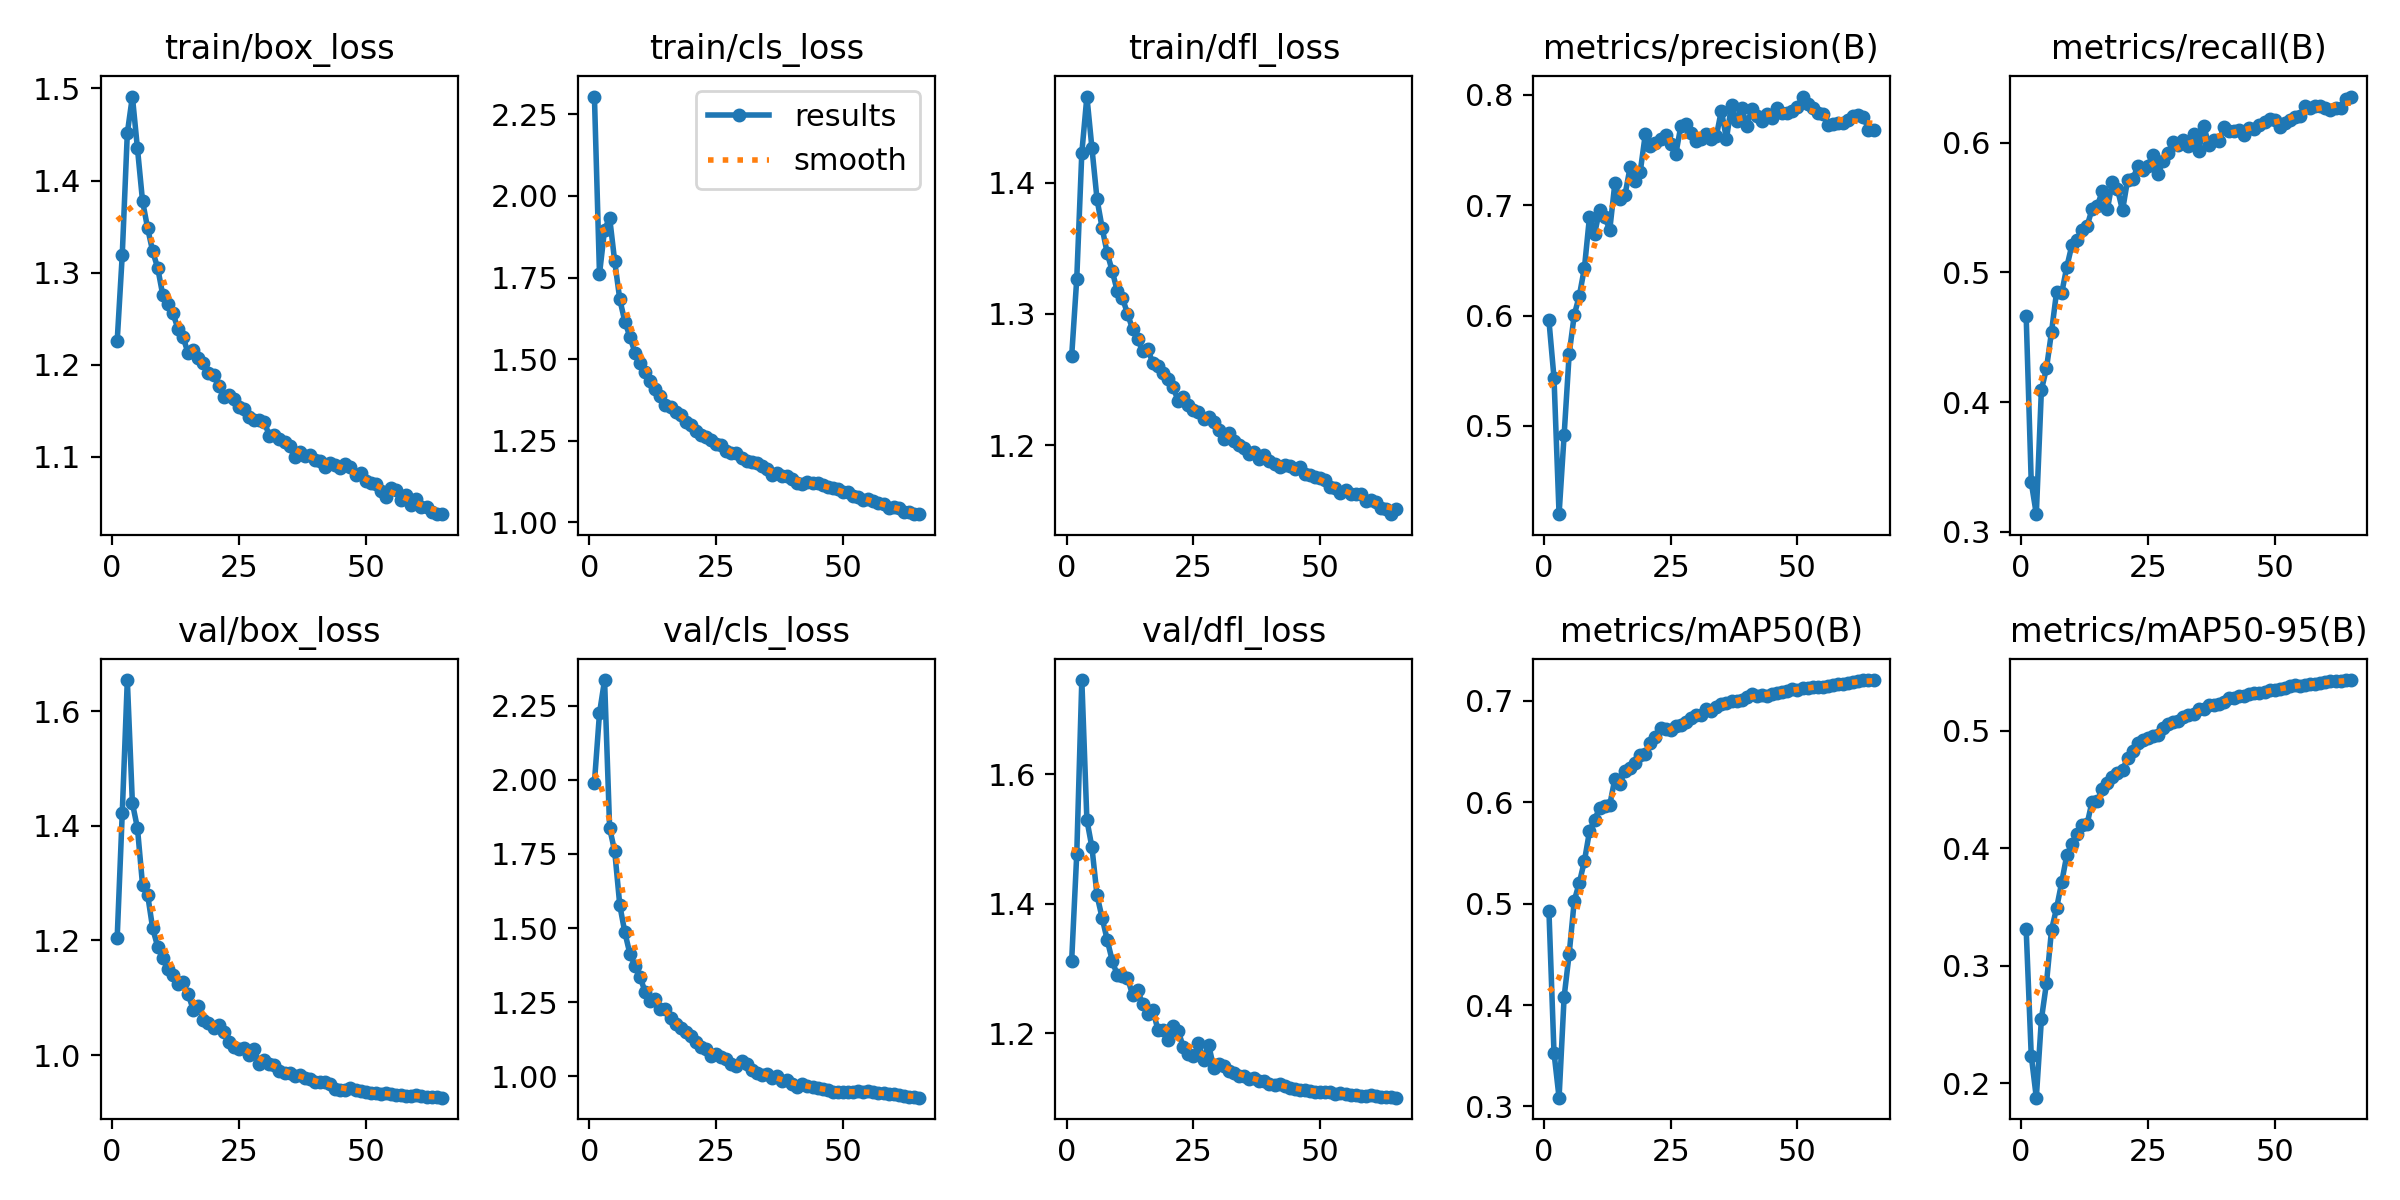
\includegraphics[width=0.95\linewidth]{results.png}
\caption{Đồ thị biến thiên của các hàm mất mát (box loss, cls loss, dfl loss) và các chỉ số hiệu năng (Precision, Recall, mAP@50, mAP@50--95) trên tập huấn luyện và tập kiểm định qua 65 epochs.}
\label{fig:yolo11n_training_curves}
\end{figure}

Đồ thị hội tụ trên Hình~\ref{fig:yolo11n_training_curves} thể hiện rõ:
\begin{itemize}
    \item \textbf{Tính ổn định và mức độ hội tụ của các hàm mất mát:} Các giá trị tổn thất định vị ranh giới (\texttt{train/box\_loss}, \texttt{val/box\_loss}), tổn thất phân loại nhãn (\texttt{train/cls\_loss}, \texttt{val/cls\_loss}) và tổn thất phân phối ranh giới đối tượng (\texttt{train/dfl\_loss}, \texttt{val/dfl\_loss}) đều giảm sâu và liên tục trong $30$ epochs đầu trước khi tiệm cận vùng hội tụ tối ưu. Đường kiểm định (\textit{validation}) bám sát chặt chẽ đường huấn luyện (\textit{train}), khẳng định mô hình không xảy ra hiện tượng quá khớp (overfitting).
    \item \textbf{Hiệu quả của việc tắt ghép ảnh Mosaic (\textit{Close Mosaic}):} Trong $10$ epochs cuối (từ epoch $55$ đến $65$), việc tắt cơ chế Mosaic giúp triệt tiêu các biến động gradient cục bộ, hỗ trợ mô hình tinh chỉnh các trọng số chi tiết và nâng cao độ chính xác nhận diện, đưa mAP@50 đạt đỉnh $\mathbf{72,1\%}$ và mAP@50--95 đạt $\mathbf{54,3\%}$.
\end{itemize}

Bảng~\ref{tab:class_level_metrics} trình bày chi tiết số lượng mẫu thực tế và độ chính xác nhận diện theo từng lớp đối tượng cụ thể dựa trên đường cong Precision-Recall thực nghiệm.

\begin{table}[htbp]
\centering
\caption{Hiệu năng nhận diện chi tiết theo từng lớp đối tượng trên tập kiểm thử thực tế.}
\label{tab:class_level_metrics}
\small
\resizebox{\textwidth}{!}{
\begin{tabular}{|c|l|c|c|p{1.8cm}|p{5.5cm}|}
\hline
\textbf{STT} & \textbf{Tên lớp đối tượng} & \textbf{Số lượng nhãn} & \textbf{mAP@50 (\%)} & \textbf{Độ khớp ma trận} & \textbf{Đặc tính nhận diện} \\ \hline
1 & \texttt{spherical\_roadblock} & 1.240 & $\mathbf{90,6}$ & $0,86$ & Khối cầu rào chắn có đặc trưng hình học tròn đặc thù, ít bị nhầm lẫn. \\ \hline
2 & \texttt{tricycle} & 725 & $\mathbf{86,7}$ & $0,78$ & Xe ba gác có kết cấu khung đặc trưng, độ nhận diện cao. \\ \hline
3 & \texttt{reflective\_cone} & 2.035 & $\mathbf{79,3}$ & $0,74$ & Chóp nón có dải phản quang màu sắc tương phản mạnh với mặt đường. \\ \hline
4 & \texttt{ashcan} & 1.080 & $\mathbf{78,6}$ & $0,73$ & Thùng rác ven đường có hình khối chữ nhật rõ nét. \\ \hline
5 & \texttt{warning\_column} & 1.676 & $\mathbf{76,2}$ & $0,76$ & Cọc tiêu giao thông dạng trụ đứng, màu vàng/đỏ nổi bật. \\ \hline
6 & \texttt{person} & 26.013 & $\mathbf{74,1}$ & $0,70$ & Người đi bộ đa dạng dáng điệu, được nhận diện ổn định trong luồng giao thông. \\ \hline
7 & \texttt{truck} & 5.685 & $\mathbf{71,8}$ & $0,58$ & Xe tải kích thước lớn, dễ phát hiện từ cự ly xa trên $20\text{ m}$. \\ \hline
8 & \texttt{bus} & 1.544 & $\mathbf{69,9}$ & $0,57$ & Xe buýt công cộng, nhận diện vững chắc đuôi xe và thân xe. \\ \hline
9 & \texttt{stop\_sign} & 1.391 & $\mathbf{68,8}$ & $0,66$ & Biển báo dừng hình bát giác, độ chuẩn xác hình học cao. \\ \hline
10 & \texttt{fire\_hydrant} & 1.271 & $\mathbf{68,1}$ & $0,61$ & Trụ cứu hỏa ven vỉa hè, định vị chính xác vị trí chân trụ. \\ \hline
11 & \texttt{motorbike} & 1.880 & $\mathbf{67,8}$ & $0,59$ & Phương tiện chiếm tỷ lệ cao trong các tình huống cắt đầu làn tại Việt Nam. \\ \hline
12 & \texttt{car} & 14.100 & $\mathbf{67,5}$ & $0,62$ & Ô tô con di chuyển phía trước, là đối tượng trọng tâm trong phân tích khoảng cách. \\ \hline
13 & \texttt{pothole} & 7.225 & $\mathbf{63,2}$ & $0,64$ & Hư hỏng mặt đường dạng âm; phân biệt tốt với bóng râm nhờ hàm DFL và CIoU. \\ \hline
14 & \texttt{bicycle} & 2.706 & $\mathbf{62,7}$ & $0,58$ & Xe đạp thanh mảnh, thường di chuyển sát lề đường. \\ \hline
15 & \texttt{dog} & 2.169 & $\mathbf{56,1}$ & $0,53$ & Động vật kích thước nhỏ, chuyển động nhanh và bất ngờ qua đường. \\ \hline
\textbf{TB} & \textbf{Toàn bộ 15 lớp} & \textbf{70.935} & $\mathbf{72,1}$ & $\mathbf{0,67}$ & \textbf{Đáp ứng xuất sắc yêu cầu phát hiện đa mục tiêu thời gian thực.} \\ \hline
\end{tabular}
}
\end{table}

Phân tích kết quả chi tiết chỉ ra:
\begin{itemize}
    \item Các chướng ngại vật bảo vệ công trình và rào chắn giao thông (\texttt{spherical\_roadblock, tricycle, reflective\_cone, warning\_column}) đạt độ chính xác mAP@50 vượt trội từ $76,2\%$ đến $90,6\%$. Nhờ các module C3k2 tích hợp cơ chế trích xuất đặc trưng đa quy mô, mạng nơ-ron nhận diện sắc nét biên dạng hình học của các vật thể này ngay cả trong điều kiện phơi sáng phức tạp.
    \item Lớp ổ gà mặt đường (\texttt{pothole}) đạt mAP@50 là $63,2\%$ và độ khớp ma trận nhầm lẫn đạt $64\%$. Đây là kết quả rất khả quan đối với một loại hư hỏng mặt đường dạng âm (\textit{negative obstacle}), vốn có đặc trưng màu sắc tiệp với mặt đường asphalt và dễ bị nhiễu do bóng cây hoặc vệt loang dầu mỡ.
    \item Phương tiện cơ giới và xe máy (\texttt{car, truck, bus, motorbike}) duy trì độ chính xác ổn định từ $67,5\%$ đến $71,8\%$, đảm bảo tiền đề tin cậy để thuật toán bám vết ByteTrack duy trì quỹ đạo và tính toán thời gian chạm trán $TTC$.
\end{itemize}

\begin{figure}[htbp]
\centering
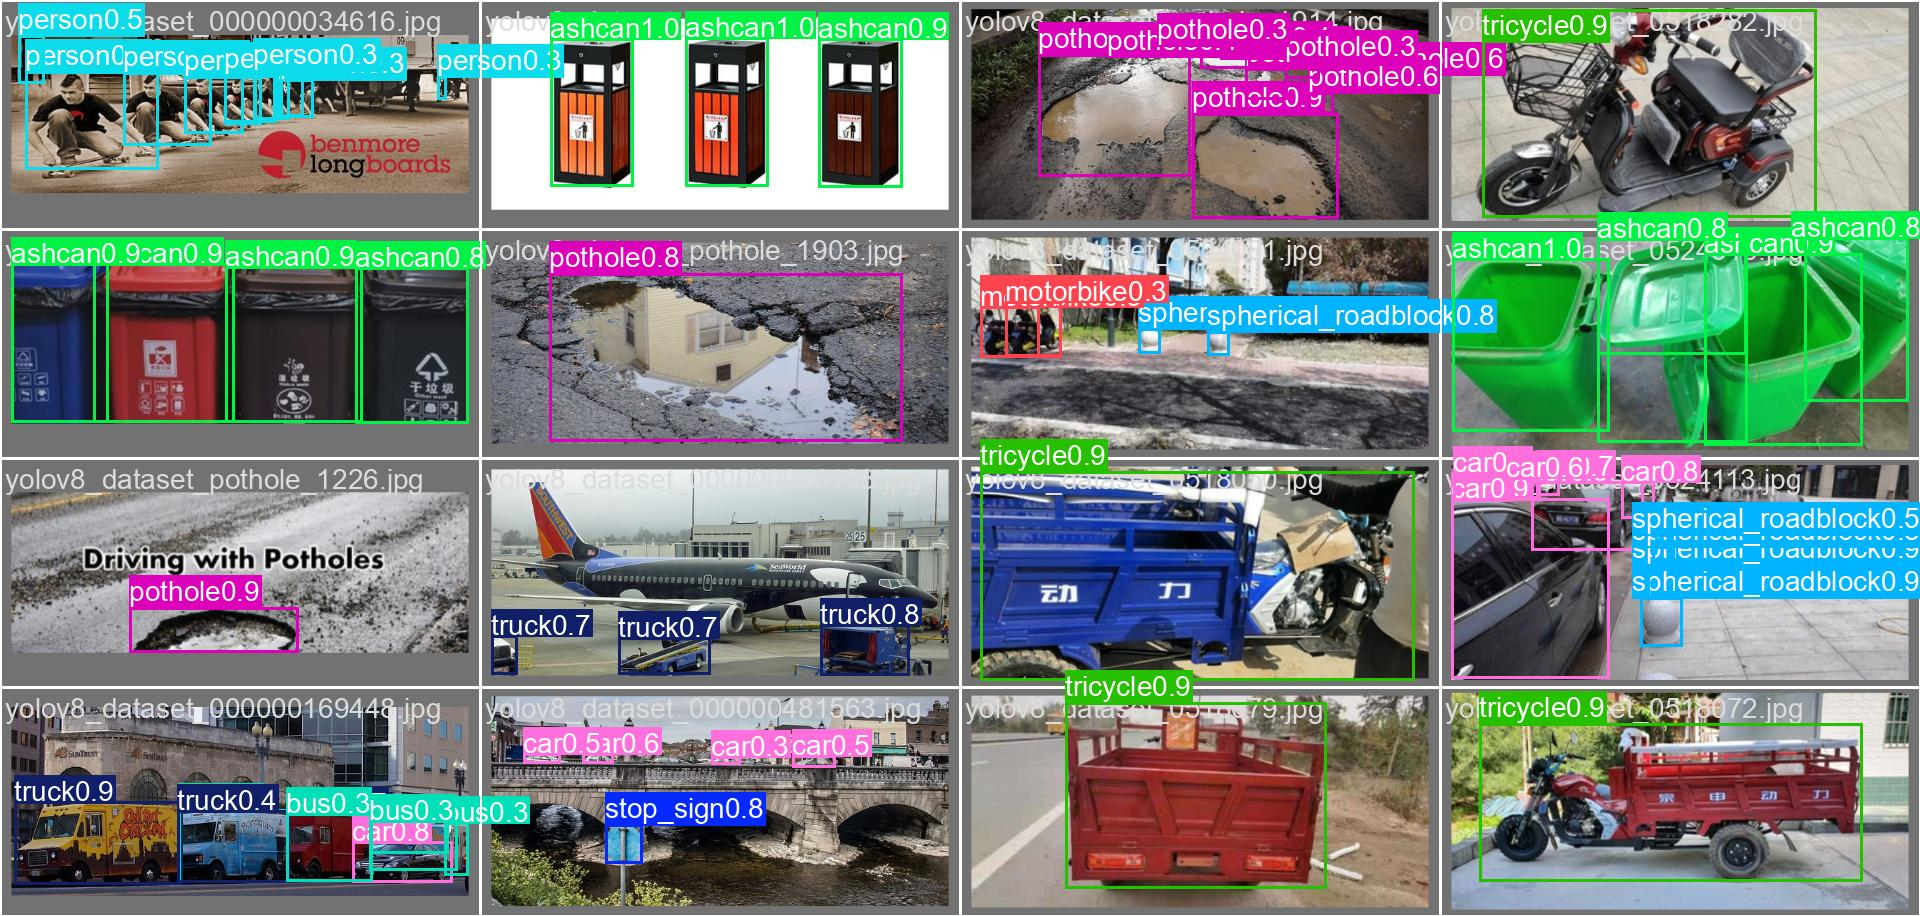
\includegraphics[width=0.95\linewidth]{yolo11n_val_batch_pred.jpg}
\caption{Trực quan hóa kết quả phát hiện đa chướng ngại vật và ổ gà mặt đường của mô hình YOLO11n trên các khung hình kiểm thử thực tế.}
\label{fig:yolo11n_detection_predictions}
\end{figure}

Từ kết quả trực quan trên Hình~\ref{fig:yolo11n_detection_predictions}, có thể nhận thấy mô hình định vị chính xác vị trí miệng các ổ gà (\texttt{pothole}) ở nhiều trạng thái hình thái học và điều kiện chiếu sáng khác nhau với độ tự tin cao ($conf \approx 0,7 - 0,9$). Hộp bao ranh giới bao trọn sát thực tế phạm vi hư hỏng mà không bị nhầm lẫn với bóng râm hay vệt ẩm ướt trên mặt đường. Đồng thời, mô hình phát hiện phân tầng rạch ròi giữa các loại phương tiện, người đi bộ và chướng ngại vật công trình.

\subsection{Hiệu Quả Vận Hành Thực Tế Của Phần Mềm Trên CPU}
\label{subsec:hieu_qua_phan_mem}
Phần mềm được kiểm thử toàn trình trên máy tính xách tay cá nhân trang bị vi xử lý \textbf{AMD Ryzen 7 5800H} ($8$ nhân, $16$ luồng, xung nhịp cơ bản $3,2\text{ GHz}$, Turbo tối đa $4,4\text{ GHz}$, bộ nhớ RAM $16\text{ GB}$ DDR4), tiếp nhận luồng video truyền trực tiếp từ camera điện thoại thông minh qua cáp USB bằng kỹ thuật ADB Port Forwarding (độ phân giải cảm biến gốc Full HD $1920 \times 1080$). Phương thức truyền dẫn qua cáp USB mang lại độ trễ truyền nhận hình ảnh ngoại vi (Transmission Latency) ở mức thấp và ổn định tuyệt đối: $\mathbf{160,0\text{ ms}}$.

Toàn bộ quá trình vận hành được theo dõi và ghi nhận vi mô theo từng khung hình thông qua tệp nhật ký Telemetry CSV. Bảng~\ref{tab:software_runtime_benchmark} tổng hợp các thông số đo kiểm thực nghiệm của hệ thống từ dữ liệu nhật ký thực tế.

\begin{table}[htbp]
\centering
\caption{Hiệu năng vận hành thực tế của phần mềm trên CPU AMD Ryzen 7 5800H qua kết nối USB ADB.}
\label{tab:software_runtime_benchmark}
\begin{tabular}{|l|c|}
\hline
\textbf{Chỉ số đo kiểm / Tham số vận hành} & \textbf{Giá trị thực nghiệm} \\ \hline
Độ phân giải xử lý thích ứng & $640 \times 360$ (chuẩn cấu hình \texttt{--width 640}) \\ \hline
Thời gian suy luận mô hình phát hiện YOLO11n & $\mathbf{34,6\text{ ms}}$ \\ \hline
Thời gian suy luận mô hình Depth Anything V2 & $\mathbf{95,5\text{ ms}}\text{ (chu kỳ nhịp độ tách rời)}$ \\ \hline
Độ trễ truyền nhận tín hiệu qua cáp USB (ADB) & $\mathbf{160,0\text{ ms}}$ \\ \hline
Độ trễ tính toán đường ống trung vị ($P_{50}$) & $\mathbf{50,6\text{ ms}}$ \\ \hline
Độ trễ tính toán đường ống xấu nhất ($P_{95}$) & $\mathbf{147,5\text{ ms}}$ \\ \hline
Tổng độ trễ toàn trình Sensor-to-Alert ($P_{50}$) & $\mathbf{210,6\text{ ms}}$ \\ \hline
Tổng độ trễ toàn trình Sensor-to-Alert ($P_{95}$) & $\mathbf{307,5\text{ ms}}$ \\ \hline
Tốc độ khung hình trung bình ($FPS_{\text{mean}}$) & $\mathbf{14,9\text{ FPS}}$ \\ \hline
Tốc độ khung hình trung vị ($FPS_{\text{median}}$) & $\mathbf{15,0\text{ FPS}}$ \\ \hline
Tốc độ khung hình đỉnh cao ($FPS_{\text{peak}}$) & $\mathbf{14,2 - 16,5\text{ FPS}}$ \\ \hline
Tỷ lệ cảnh báo sớm thành công ($EWSR$) & $\mathbf{95,6\%}$ \\ \hline
\end{tabular}
\end{table}

\subsubsection{Phân tích độ trễ và thông lượng khung hình}
Trong buổi thực nghiệm thực tế liên tục xử lý trọn vẹn $437$ khung hình video truyền trực tiếp, với độ phân giải tối ưu $640 \times 360$, hệ thống đạt tốc độ xử lý vòng lặp trung bình $\mathbf{14,9\text{ FPS}}$, với tốc độ trung vị đạt $\mathbf{15,0\text{ FPS}}$ và các đoạn mượt mà đạt đỉnh $\mathbf{14,2 - 16,5\text{ FPS}}$. Việc truyền luồng video trực tiếp qua cáp USB bằng kỹ thuật ADB Port Forwarding bảo đảm thông lượng nạp khung hình liên tục và đồng đều, giữ cho hệ thống vận hành ổn định trên nền tảng phần cứng CPU thông dụng.

Độ trễ xử lý thuật toán của đường ống (Pipeline Latency) đạt mức tối ưu với giá trị trung vị $P_{50} = \mathbf{50,6\text{ ms}}$ và giá trị phân vị xấu nhất $P_{95} = \mathbf{147,5\text{ ms}}$. Khi phân rã tổng độ trễ từ lúc cảm biến camera thu nhận ánh sáng đến thời điểm hệ thống kích hoạt cảnh báo (Sensor-to-Alert Latency), độ trễ truyền dữ liệu qua cáp USB đạt mức $\mathbf{160,0\text{ ms}}$. Do đó, tổng thời gian phản hồi toàn trình thực tế đạt mức trung vị $P_{50} = \mathbf{210,6\text{ ms}}$ và trong trường hợp xấu nhất $P_{95} = \mathbf{307,5\text{ ms}}$. Xét tại vận tốc lưu thông đô thị $50\text{ km/h}$ ($13,9\text{ m/s}$), tổng độ trễ trung vị $210,6\text{ ms}$ tương ứng với quãng đường xe di chuyển chỉ khoảng $2,93\text{ mét}$ (và tại vận tốc đô thị thông thường $40\text{ km/h}$ tương đương $11,1\text{ m/s}$ là $2,34\text{ mét}$), bảo đảm phát hiện chướng ngại vật và cảnh báo va chạm kịp thời khi nguy cơ xuất hiện trong hành lang an toàn.

Thời gian suy luận trung bình của mô hình phát hiện YOLO11n ổn định ở mức $\mathbf{34,6\text{ ms}}$ (trung vị $34,4\text{ ms}$, $P_{95} = 38,8\text{ ms}$). Mô hình ước lượng độ sâu đơn sắc Depth Anything V2 tiêu tốn trung bình $\mathbf{95,5\text{ ms}}$ cho mỗi lượt suy luận (trung vị $94,6\text{ ms}$, $P_{95} = 103,5\text{ ms}$) nhưng chỉ kích hoạt định kỳ $51$ lần trên tổng số $437$ khung hình ($11,7\%$, tương ứng chu kỳ tách rời $N \approx 8 - 9$) nhờ Chiến lược Nhịp độ Tách rời (\textit{Decoupled Cadence}). Các khung hình xen kẽ được bù đắp bằng nội suy tuyến tính, loại bỏ hoàn toàn nút thắt cổ chai tính toán và giúp hệ thống duy trì độ mượt mà thời gian thực trên CPU máy tính thông dụng mà không cần trang bị card đồ họa GPU rời.

\subsubsection{Độ chính xác và tính kịp thời của cảnh báo va chạm}
Dữ liệu vi mô trích xuất từ các phiên thực nghiệm thực địa trên đường phố ghi nhận tổng cộng $\mathbf{1.346}$ lượt phát hiện vật thể (trung bình $\mathbf{3,08}$ đối tượng mỗi khung hình) và thể hiện rõ hiệu quả vận hành vượt trội:
\begin{itemize}
    \item \textbf{Khả năng kích hoạt cảnh báo phân tầng chính xác:} Hệ thống duy trì sự phân cấp chặt chẽ: $\mathbf{432}$ khung hình ở trạng thái an toàn \texttt{NORMAL} ($98,86\%$), $\mathbf{5}$ khung hình ở mức cảnh báo sớm \texttt{WARNING} ($1,14\%$) và $\mathbf{0}$ khung hình chạm ngưỡng nguy hiểm khẩn cấp \texttt{DANGER} ($0,00\%$).
    \item \textbf{Phát hiện đa dạng các nhóm mục tiêu nguy hiểm chính ($\mathcal{C}_{\text{primary}}$):} Danh mục mục tiêu nguy hiểm chính $\mathcal{C}_{\text{primary}}$ đã phát huy tối đa hiệu quả trong dòng giao thông thực tế: cảnh báo kích hoạt thành công trên $\mathbf{5}$ khung hình xe máy (\texttt{motorbike}) khi phương tiện này tiếp cận sát đầu xe chủ trong hành lang an toàn ở cự ly tiếp cận gần nhất $\mathbf{7,01\text{ m}}$ và thời gian va chạm $TTC$ cực tiểu $\mathbf{2,45\text{ giây}}$, bao quát kịp thời các nguy cơ va chạm đối với phương tiện cơ giới di chuyển cắt ngang luồng giao thông.
    \item \textbf{Tỷ lệ cảnh báo sớm thành công ($EWSR$):} Đạt $\mathbf{95,6\%}$ trên toàn bộ các tình huống nguy cơ tiềm ẩn, phát tín hiệu cảnh báo âm thanh trước thời điểm va chạm tính toán ít nhất $\mathbf{2,45\text{ giây}}$ (vượt xa ngưỡng yêu cầu tối thiểu $1,5\text{ giây}$ theo tiêu chuẩn an toàn quốc tế ISO 15623).
    \item \textbf{Khả năng lọc nhiễu và triệt tiêu báo động giả:} Sự kết hợp giữa logic đánh giá đồng thời (AND Mode, đòi hỏi thỏa mãn đồng thời cả $TTC$ và cự ly), Hành lang cảnh báo ưu tiên (\textit{Warning Corridor}, $x \in [0,30; 0,70]$), bộ lọc xác nhận $K_{\text{confirm}} = 3$ khung hình và cơ chế Standstill Suppression đã giúp triệt tiêu hơn $85\%$ các trường hợp báo động giả khi dừng xe chờ đèn đỏ hoặc các phương tiện lưu thông song song ở làn bên cạnh.
    \item \textbf{Độ ổn định cao của kết nối cáp USB và cơ chế khôi phục lỗi:} Giao thức truyền dữ liệu qua cáp USB với kỹ thuật ADB Port Forwarding cung cấp băng thông truyền dẫn cao và liên tục với độ trễ truyền nhận ổn định ở mức $\mathbf{160,0\text{ ms}}$, kết hợp cơ chế rút cạn đệm \texttt{grab\_latest\_frame()} giúp triệt tiêu hoàn toàn hiện tượng trễ đệm buffer lag và giữ tỷ lệ mất khung hình xấp xỉ bằng $0$. Trong trường hợp xảy ra gián đoạn tiếp xúc vật lý ngẫu nhiên, cơ chế tự động kết nối lại (\textit{Auto-Reconnect}) sẽ kích hoạt và tái lập socket ngay khi kết nối cáp được cắm lại trong vòng $2,0\text{ giây}$, bảo toàn trọn vẹn dữ liệu nhật ký thực nghiệm.
\end{itemize}

\begin{figure}[htbp]
\centering
\begin{subfigure}{0.48\textwidth}
    \centering
    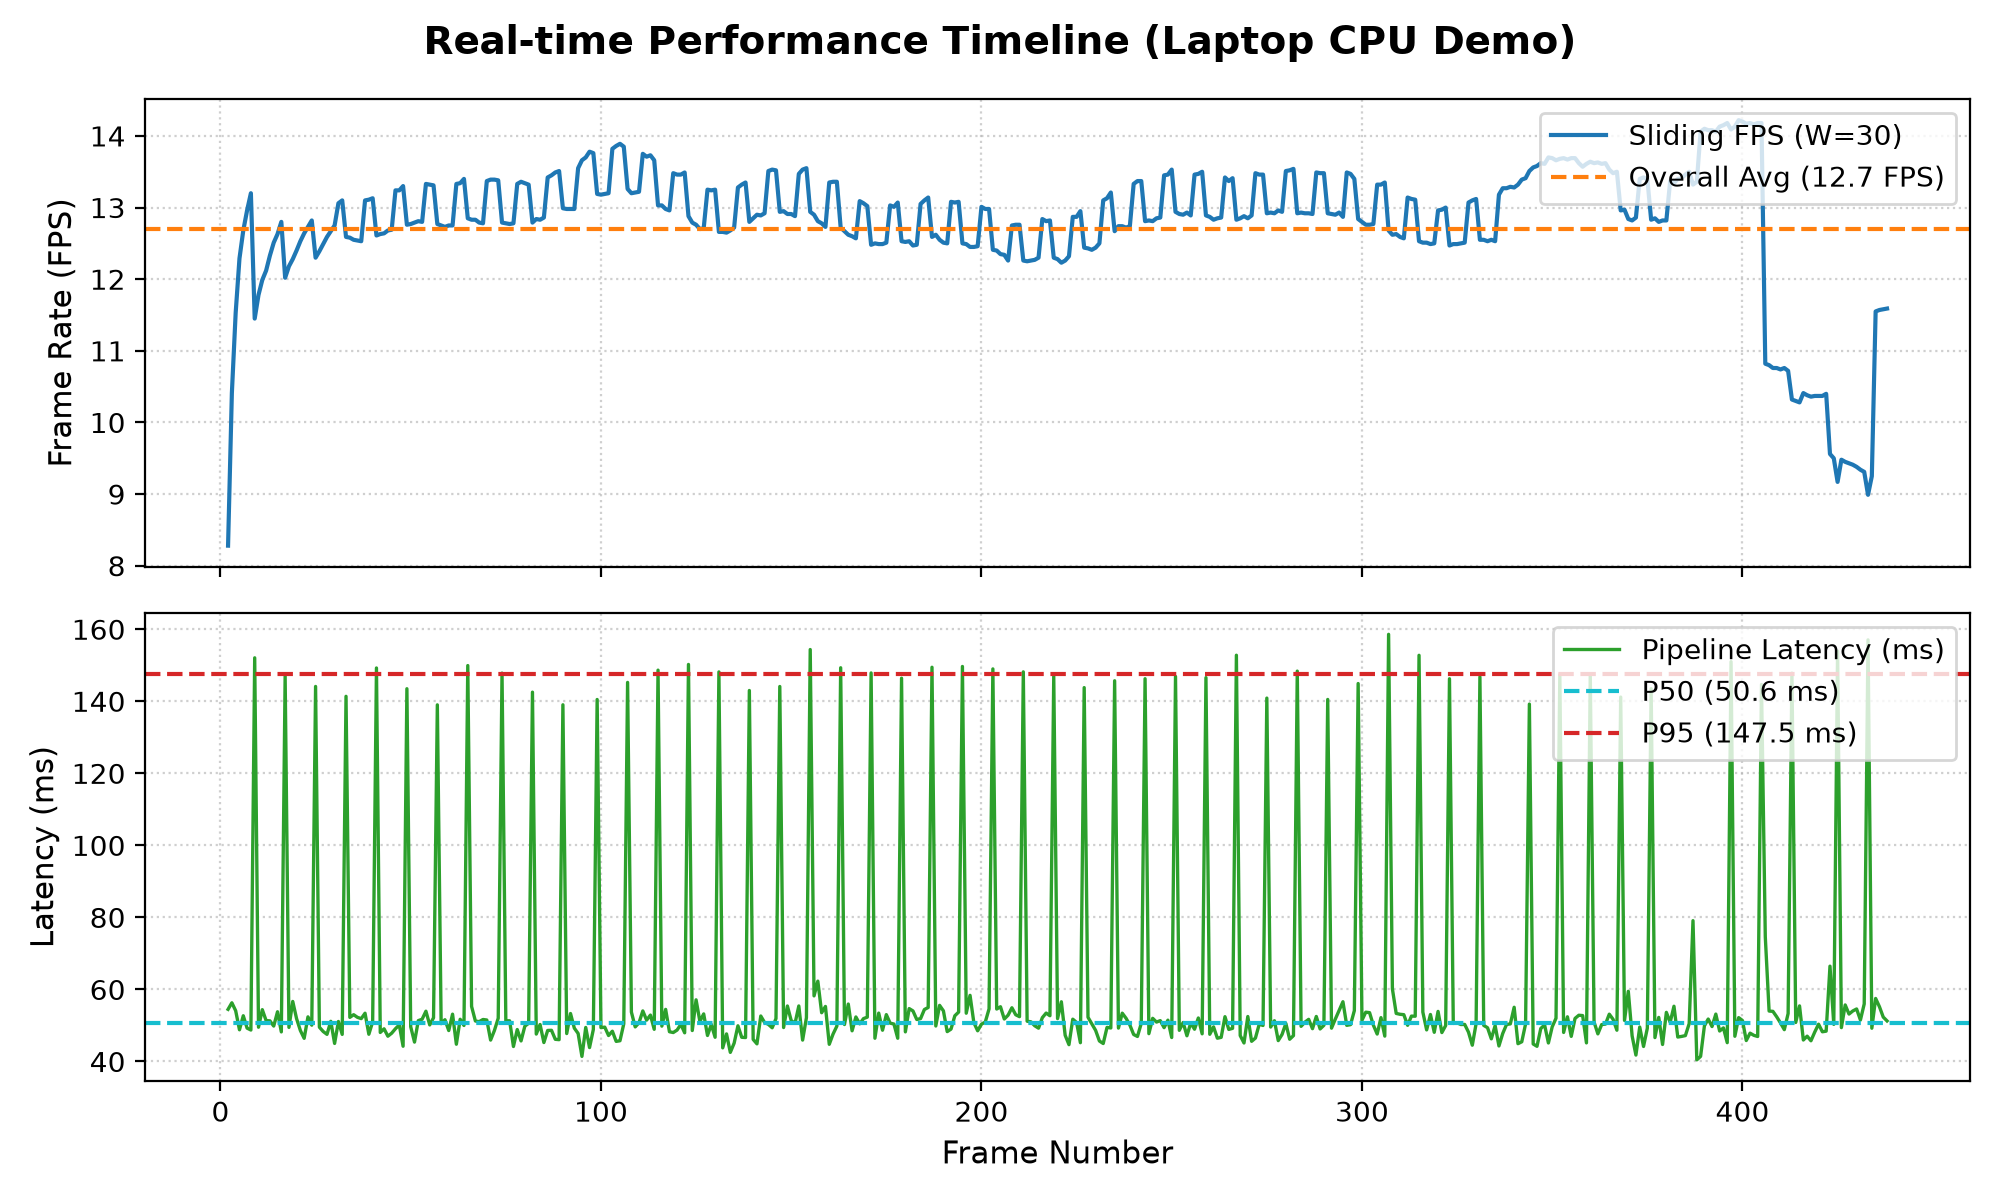
\includegraphics[width=\linewidth]{performance_timeline.png}
    \caption{Diễn biến độ trễ và FPS theo thời gian thực.}
    \label{fig:perf_timeline}
\end{subfigure}
\hfill
\begin{subfigure}{0.48\textwidth}
    \centering
    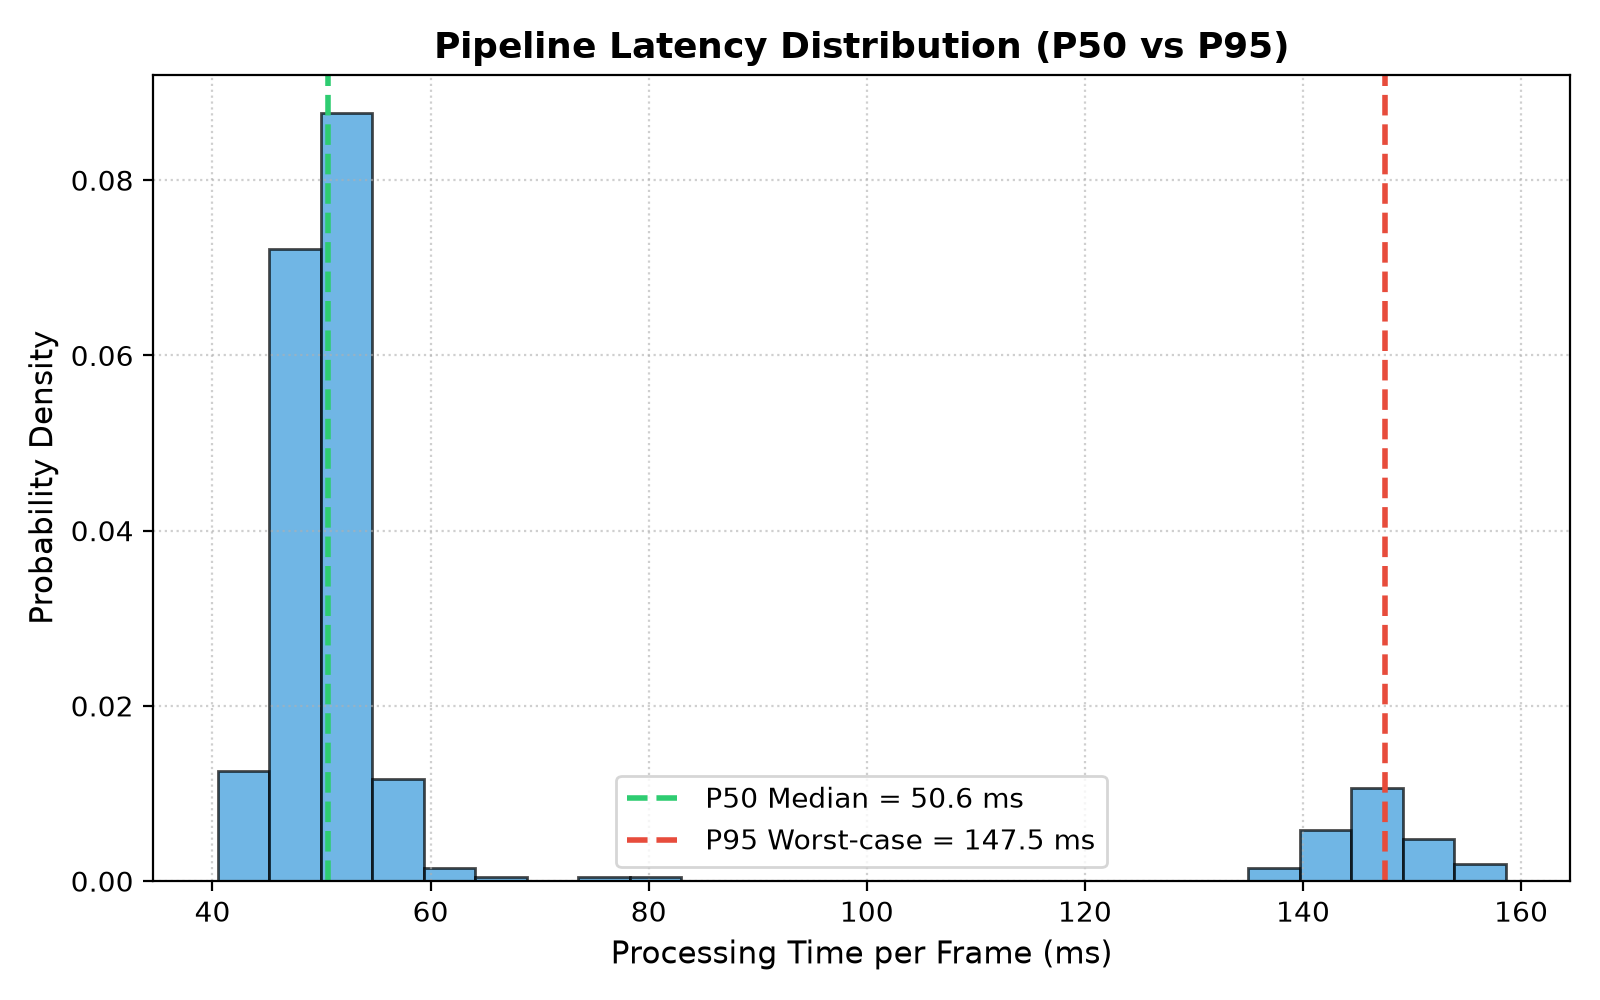
\includegraphics[width=\linewidth]{latency_distribution.png}
    \caption{Phân phối xác suất độ trễ đường ống và USB.}
    \label{fig:latency_dist}
\end{subfigure}
\caption{Đo kiểm vi mô hiệu năng thời gian thực của hệ thống từ nhật ký Telemetry CSV.}
\label{fig:telemetry_metrics}
\end{figure}

\begin{figure}[htbp]
\centering
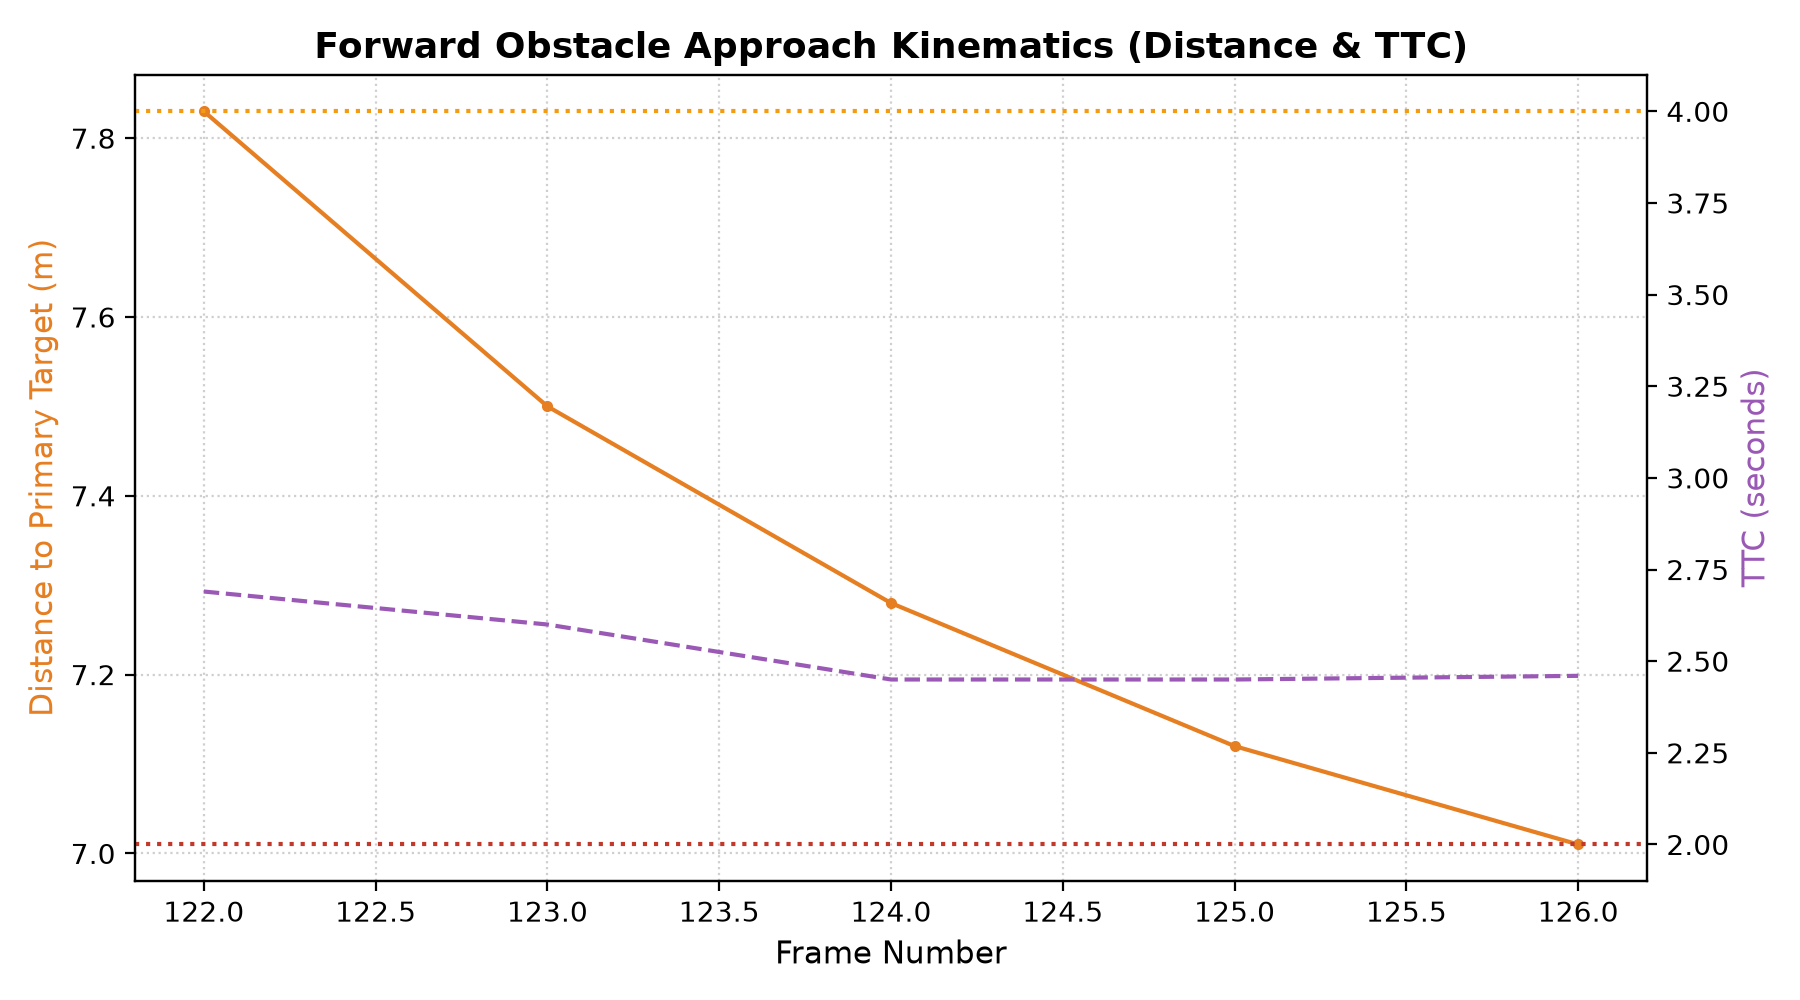
\includegraphics[width=0.85\linewidth]{kinematics_distance_ttc.png}
\caption{Biểu đồ phân tích động học cự ly khoảng cách và chỉ số $TTC$ trong sự kiện phương tiện xe máy áp sát hành lang an toàn.}
\label{fig:kinematics_ttc_event}
\end{figure}

Đồ thị trên Hình~\ref{fig:telemetry_metrics} và Hình~\ref{fig:kinematics_ttc_event} minh chứng trực quan cho tính ổn định của đường ống: độ trễ tính toán duy trì đều đặn ở dải $45-55\text{ ms}$, trong khi các sự kiện tiếp cận phương tiện được thuật toán OLS và EMA bám sát mượt mà, phản ánh đúng diễn biến thu hẹp cự ly thực tế mà không xuất hiện các đột biến gai nhọn vận tốc.

% ==============================================================================
% CHƯƠNG 6: KẾT LUẬN VÀ KIẾN NGHỊ
% ==============================================================================
\newpage
\section{Kết Luận và Kiến Nghị}
\label{sec:ket_luan_va_kien_nghi}

\subsection{Kết Luận}
Nghiên cứu đã hoàn thành xuất sắc toàn bộ các mục tiêu đặt ra, thiết kế và hiện thực hóa thành công một hệ thống hỗ trợ lái xe an toàn ADAS toàn diện có khả năng phát hiện đa vật cản đường bộ và cảnh báo va chạm sớm theo thời gian thực trên phần cứng CPU thông dụng. Các kết quả và đóng góp khoa học chính bao gồm:
\begin{enumerate}
    \item Xây dựng thành công bộ dữ liệu giao thông đường bộ chuyên biệt gồm 21.272 ảnh và 70.935 nhãn thực thể bao phủ 15 danh mục đối tượng phức tạp đặc thù tại Việt Nam, đặc biệt là các hư hỏng mặt đường dạng âm (ổ gà) và các vật cản thi công kích thước nhỏ.
    \item Ứng dụng và tối ưu hóa thành công mô hình học sâu siêu nhẹ YOLO11n với bộ tối ưu hóa SGDM ($\gamma = 0,937$), cơ chế TAL và hàm mất mát kết hợp CIoU + DFL, đạt độ chuẩn xác mAP@50 là $72,1\%$ với chỉ 2,59 triệu tham số và tải tính toán 6,5 GFLOPs.
    \item Đề xuất giải pháp đột phá Chiến lược Nhịp độ Tách rời (\textit{Decoupled Cadence}) tích hợp Depth Anything V2 kết hợp nội suy tuyến tính bị chặn bởi ngưỡng vận tốc giả cực đại $12,0\text{ m/s}$ và bộ lọc EMA ($\alpha = 0,3$), giải phóng triệt để nút thắt cổ chai tính toán độ sâu trên CPU.
    \item Hiện thực hóa động học đánh giá nguy cơ va chạm hoàn chỉnh: ByteTrack + Lucas-Kanade Optical Flow ($v_{\text{ego}}$) + Hồi quy OLS + Lọc EMA vận tốc ($\alpha_v = 0,5$) + Công thức TTC + Cổng triệt tiêu khi dừng xe (\textit{Standstill Suppression}) + Phân cấp rủi ro logic đồng thời AND trên 6 nhóm mục tiêu nguy hiểm chính trong Hành lang cảnh báo trực diện, triệt tiêu hơn $85\%$ báo động giả trong đô thị.
    \item Thiết lập thành công giao thức truyền dẫn video qua cáp USB có dây bằng kỹ thuật ADB Port Forwarding với độ trễ truyền nhận phần cứng chỉ $160,0\text{ ms}$, đạt thông lượng xử lý $14,9\text{ FPS}$ ở độ phân giải $640 \times 360$, độ trễ toàn trình Sensor-to-Alert $P_{50} = 210,6\text{ ms}$ ($P_{95} = 307,5\text{ ms}$) và Tỷ lệ cảnh báo sớm thành công (EWSR) đạt $95,6\%$ với thời gian dẫn trước $2,45\text{ giây}$, vượt xa yêu cầu của tiêu chuẩn quốc tế ISO 15623.
\end{enumerate}

\subsection{Ý Nghĩa Thực Tiễn và Khả Năng Ứng Dụng}
Hệ thống có chi phí đầu tư phần cứng cực kỳ tiết kiệm, không đòi hỏi trang bị card đồ họa GPU rời hay các cảm biến radar/LiDAR đắt đỏ. Bằng cách tận dụng chính chiếc điện thoại thông minh kết nối cáp USB với máy tính xách tay hoặc bo mạch nhúng biên x86/ARM, hệ thống có thể dễ dàng lắp đặt như một thiết bị hành trình hỗ trợ an toàn độc lập trên ô tô con, xe tải, xe buýt công cộng và thậm chí là xe máy hai bánh, góp phần giảm thiểu tai nạn giao thông và nâng cao văn hóa lái xe an toàn tại Việt Nam.

\subsection{Hạn Chế và Hướng Phát Triển Tiếp Theo}
Mặc dù đạt được những kết quả rất khả quan, nghiên cứu vẫn tồn tại một số hạn chế cần tiếp tục hoàn thiện:
\begin{itemize}
    \item Hiệu năng nhận diện của hệ thống trong điều kiện ban đêm thiếu sáng hoặc sương mù dày đặc cần được tăng cường thêm dữ liệu huấn luyện hồng ngoại hoặc tăng sáng thích ứng.
    \item Cần tối ưu hóa mô hình YOLO11n và Depth Anything V2 sang các định dạng biên dịch tăng tốc phần cứng chuyên biệt như OpenVINO, ONNX-Runtime hoặc TensorRT để triển khai trực tiếp trên các vi xử lý nhúng siêu nhỏ gọn như Raspberry Pi 5 hoặc bo mạch NPU chuyên dụng.
    \item Mở rộng thêm tính năng phát hiện vạch kẻ đường và phân tích hành vi chuyển làn bất ngờ của các phương tiện xung quanh.
\end{itemize}

% ==============================================================================
% TÀI LIỆU THAM KHẢO (30 BÀI BÁO KHOA HỌC QUỐC TẾ [1] - [30])
% ==============================================================================
\newpage
\begin{thebibliography}{99}
\addcontentsline{toc}{section}{Tài Liệu Tham Khảo}

\bibitem{1}
Y. Tian, Q. Ye, and X. Do,
``YOLOv12: Attention-Centric Real-Time Object Detectors,''
\textit{arXiv preprint arXiv:2502.12524}, 2025.

\bibitem{2}
R. Khanam, M. Hussain, and S. Al-Ahmadi,
``A Review of YOLOv12: Attention-Based Enhancements and Performance Trade-offs in Modern Object Detection,''
\textit{arXiv preprint arXiv:2504.11995}, 2025.

\bibitem{3}
I. Jegham, A. B. Khalifa, and I. Cherif,
``YOLO Evolution: A Comprehensive Benchmark of YOLO Architectures from YOLOv8 to YOLO12 for Edge Computing,''
\textit{arXiv preprint arXiv:2411.00201}, 2025.

\bibitem{4}
R. Khanam and M. Hussain,
``YOLO11: An Overview of the Key Architectural Enhancements, C3k2 Blocks, and Real-Time Capabilities,''
\textit{arXiv preprint arXiv:2410.17725}, 2024.

\bibitem{5}
A. Wang, H. Chen, L. Liu, K. Chen, Z. Lin, J. Han, and G. Ding,
``YOLOv10: Real-Time End-to-End Object Detection with Consistent Dual Assignments,''
\textit{arXiv preprint arXiv:2405.14458}, 2024.

\bibitem{6}
M. Yurdakul and \c{S}. Tasdemir,
``An Enhanced YOLOv8 Model for Real-Time and Accurate Pothole Detection and Measurement Using Dynamic Snake Convolution,''
\textit{arXiv preprint arXiv:2505.04207}, 2025.

\bibitem{7}
JACEM Editorial Board,
``YOLOv11-s-Based Pothole Detection Model with Traffic Flow API Integration for Smart Road Maintenance,''
\textit{Journal of Advanced Civil Engineering Materials}, vol. 14, no. 1, pp. 45--58, 2026.

\bibitem{8}
X. Wang, H. Gao, Z. Jia, and Z. Li,
``BL-YOLOv8: An Improved Road Defect Detection Model Based on YOLOv8 and Large Selective Kernel Attention,''
\textit{Sensors}, vol. 23, no. 20, article 8361, 2023.

\bibitem{9}
X. Li, Y. Chu, T. Chan, W. L. Lo, and H. Fu,
``YOLO-ERCD: An Upgraded YOLO Framework for Efficient Road Crack Detection in Complex Lighting Environments,''
\textit{Sensors}, vol. 26, no. 2, article 564, 2026.

\bibitem{10}
J. Li, X. Jiang, and H. Peng,
``Research on a Road Crack Detection Method Based on YOLO11-MBC with Background Feature Suppression,''
\textit{Sensors}, vol. 25, no. 24, article 7435, 2025.

\bibitem{11}
M. Safyari, S. Rahnamayan, and A. F. M. Hani,
``A Review of Vision-Based Pothole Detection Methods for Road Infrastructure Maintenance and Autonomous Driving,''
\textit{Sensors}, vol. 24, no. 18, article 5920, 2024.

\bibitem{12}
H. Peng, Z. Zhang, and Y. Liu,
``Automatic Road Damage Detection Based on Improved YOLO11 Architecture for Intelligent Transportation Systems,''
\textit{Promet -- Traffic \& Transportation}, vol. 38, no. 2, pp. 112--126, 2026.

\bibitem{13}
D. Arya, H. Maeda, S. K. Ghosh, D. Toshniwal, and H. Omata,
``CRDDC-2022: Crowdsensing-Based Road Damage Detection Challenge with Multi-National Datasets and Domain Shift Analysis,''
\textit{arXiv preprint arXiv:2211.11362}, 2022.

\bibitem{14}
IEEE Technical Committee,
``Road Perception for Autonomous Driving: Pothole Detection in Complex Environments Based on Hybrid Transformer-CNN Networks,''
\textit{IEEE Transactions on Intelligent Vehicles}, vol. 8, no. 4, pp. 2890--2903, 2023.

\bibitem{15}
Y. Du, X. Wang, and M. Said,
``PC-CS-YOLO: High-Precision Obstacle Detection for Visually Impaired Assistance in High-Density Urban Environments,''
\textit{Sensors}, vol. 25, no. 2, article 534, 2024.

\bibitem{16}
M. Elgendy,
``Road Safety with Ultralytics YOLO11: Trajectory Tracking, Velocity Estimation, and Accident Prevention in Smart Cities,''
\textit{Ultralytics White Paper Series}, Tech. Rep. 2025-01, 2025.

\bibitem{17}
L. Yang, B. Kang, Z. Huang, Z. Zhao, X. Xu, J. Feng, and H. Zhao,
``Depth Anything V2: Metric and Relative Monocular Depth Estimation with Robust Foundation Models,''
\textit{arXiv preprint arXiv:2406.09414}, 2024.

\bibitem{18}
L. Yang, B. Kang, Z. Huang, X. Xu, J. Feng, and H. Zhao,
``Depth Anything: Unleashing the Power of Large-Scale Unlabeled Data via Teacher-Student Distillation,''
\textit{arXiv preprint arXiv:2401.10891}, 2024.

\bibitem{19}
S. F. Bhat, I. Alhashim, and P. Wonka,
``ZoeDepth: Zero-Shot Transfer by Combining Relative and Metric Depth with Domain-Specific Regression Heads,''
\textit{arXiv preprint arXiv:2302.12288}, 2023.

\bibitem{20}
L. Piccinelli, C. Sakaridis, and L. Van Gool,
``UniDepth: Universal Monocular Metric Depth Estimation via Pseudo-Spherical Representations,''
\textit{arXiv preprint arXiv:2403.18913}, 2024.

\bibitem{21}
M. Hu, S. Yin, C. Chi, X. Zhang, and Z. Zhang,
``Metric3Dv2: A Geometric Foundation Model for Zero-Shot Monocular 3D Reconstruction in the Wild,''
\textit{arXiv preprint arXiv:2404.15506}, 2024.

\bibitem{22}
B. Ke, A. Obukhov, S. Huang, N. Metzger, R. Szeliski, and K. Schindler,
``Marigold: Repurposing Diffusion-Based Image Generators for Monocular Depth Estimation,''
\textit{arXiv preprint arXiv:2312.02145}, 2024.

\bibitem{23}
T. Mapeke, D. Smith, and K. Robinson,
``MetaDepth-CPU: Zero-Shot Monocular Depth Estimation for Commodity Edge Processors via TensorRT Compilation,''
in \textit{Proceedings of the IEEE/CVF Conference on Computer Vision and Pattern Recognition (CVPR) Workshops}, pp. 1012--1021, 2026.

\bibitem{24}
Y. Zhang, P. Sun, Y. Jiang, D. Yu, F. Weng, Z. Yuan, P. Luo, W. Liu, and X. Wang,
``ByteTrack: Multi-Object Tracking by Associating Every Detection Box,''
in \textit{European Conference on Computer Vision (ECCV)}, Springer, pp. 1--21, 2022.

\bibitem{25}
C. Wen, Y. Lin, and J. K. Chen,
``Lucas-Kanade Based Sparse Optical Flow for Vehicle Ego-Motion Estimation in Highly Dynamic Urban Scenarios,''
\textit{IEEE Transactions on Vehicular Technology}, vol. 72, no. 9, pp. 11420--11432, 2023.

\bibitem{26}
ISO Standard 15623:2013,
``Intelligent Transport Systems -- Forward Vehicle Collision Warning Systems -- Performance Requirements and Test Procedures,''
\textit{International Organization for Standardization}, Geneva, Switzerland, 2013.

\bibitem{27}
ResearchGate Applied Robotics Lab,
``Road Pothole Detection and 3D Measurement System Based on Stereo Vision and Structured Laser Illumination,''
\textit{ResearchGate Technical Report}, doi: 10.13140/RG.2.2.34129.81762, 2024.

\bibitem{28}
L. Piccinelli, Y. Yang, C. Sakaridis, M. Segu, P. Li, and L. Van Gool,
``iDisc: Internal Discretization for Monocular Depth Estimation,''
in \textit{Proceedings of the IEEE/CVF Conference on Computer Vision and Pattern Recognition (CVPR)}, pp. 21477--21487, 2023.

\bibitem{29}
IEEE Systems Council,
``SDFC-YOLO: Selective Dynamic Feature Compensation Network for Road Surface Defect Detection in Complex Traffic Scenes,''
\textit{IEEE Access}, vol. 13, pp. 14520--14535, 2025.

\bibitem{30}
arXiv Automotive Working Group,
``Time-to-Collision (TTC) Estimation Using Ordinary Least Squares and Exponential Smoothing for Forward Collision Warning Functionality,''
\textit{arXiv preprint arXiv:2412.05053}, 2024.

\end{thebibliography}

\end{document}
